%% This is a sample manuscript marked up using the
%% AASTeX v5.x LaTeX 2e macros.

%% The first piece of markup in an AASTeX v5.x document
%% is the \documentclass command. LaTeX will ignore
%% any data that comes before this command.

%% The command below calls the preprint style
%% which will produce a one-column, single-spaced document.
%% Examples of commands for other substyles follow. Use
%% whichever is most appropriate for your purposes.
%%

%\documentclass[11pt,preprint2]{aastex}
% manuscript produces a one-column, double-spaced document:
%\documentclass[manuscript]{aastex}
%% preprint2 produces a double-column, single-spaced document:

\documentclass{emulateapj}
%\documentclass[preprint]{aastex}

\usepackage{natbib}
\usepackage{amsmath}
\bibliographystyle{apj}
\usepackage{graphicx}

\usepackage{color}
\usepackage[normalem]{ulem}
\usepackage{url}

\DeclareUrlCommand\ULurl{%
  \renewcommand\UrlFont{\ttfamily\color{blue}}%
  \renewcommand\UrlLeft{\bgroup}%
  \renewcommand\UrlRight{\egroup}}


\newcommand{\mintext}{\text{min}}
\newcommand{\maxtext}{\text{max}}
\newcommand{\rad}{\text{rad}}
\newcommand{\IR}{\text{IR}}
\newcommand{\ir}{\text{IR}}
\newcommand{\therm}{\text{therm}}
\newcommand{\cosmo}{\text{cosmo}}
\newcommand{\fg}{\text{fg}}
\newcommand{\res}{\text{res}}
\newcommand{\shot}{\text{shot}}
\newcommand{\SNR}{\text{SNR}}

\newcommand{\Fb}{\mathbf{F}}
\newcommand{\Mb}{\mathbf{M}}
\newcommand{\Cb}{\mathbf{C}}
\newcommand{\Ab}{\mathbf{A}}
\newcommand{\xb}{\mathbf{x}}
\newcommand{\pb}{\mathbf{p}}
\newcommand{\qb}{\mathbf{q}}
\newcommand{\Wb}{\mathbf{W}}


%% Sometimes a paper's abstract is too long to fit on the
%% title page in preprint2 mode. When that is the case,
%% use the longabstract style option.

%% \documentclass[preprint2,longabstract]{aastex}

%% If you want to create your own macros, you can do so
%% using \newcommand. Your macros should appear before
%% the \begin{document} command.
%%
%% If you are submitting to a journal that translates manuscripts
%% into SGML, you need to follow certain guidelines when preparing
%% your macros. See the AASTeX v5.x Author Guide
%% for information.

%% You can insert a short comment on the title page using the command below.

%\slugcomment{Not to appear in Nonlearned J., 45.}

%% If you wish, you may supply running head information, although
%% this information may be modified by the editorial offices.
%% The left head contains a list of authors,
%% usually a maximum of three (otherwise use et al.).  The right
%% head is a modified title of up to roughly 44 characters.
%% Running heads will not print in the manuscript style.

\shorttitle{Foreground and sensitivity analysis for 21cm/Infrared studies}
\shortauthors{Neben et al.}

%% This is the end of the preamble.  Indicate the beginning of the
%% paper itself with \begin{document}.



\begin{document}

\title{Foreground and sensitivity analysis for broad band 21\,cm--Ly$\alpha$ and 21\,cm--H$\alpha$ correlation experiments probing the Epoch of Reionization}

%% Use \author, \affil, and the \and command to format
%% author and affiliation information.
%% Note that \email has replaced the old \authoremail command
%% from AASTeX v4.0. You can use \email to mark an email address
%% anywhere in the paper, not just in the front matter.
%% As in the title, use \\ to force line breaks.

\author{Abraham R. Neben\altaffilmark{1},
Brian Stalder\altaffilmark{2},
John L. Tonry\altaffilmark{2},
Jacqueline N. Hewitt\altaffilmark{1}}

\affil{\altaffilmark{1}MIT Kavli Institute, Massachusetts Institute of Technology, Cambridge, MA, 02139 USA}
\affil{\altaffilmark{2}Institute for Astronomy, University of Hawaii, 2680 Woodlawn Drive, Honolulu HI 96822}

%% Notice that each of these authors has alternate affiliations, which
%% are identified by the \altaffilmark after each name.  Specify alternate
%% affiliation information with \altaffiltext, with one command per each
%% affiliation.

%% Mark off your abstract in the ``abstract'' environment. In the manuscript
%% style, abstract will output a Received/Accepted line after the
%% title and affiliation information. No date will appear since the author
%% does not have this information. The dates will be filled in by the
%% editorial office after submission.

\begin{abstract}
NEED TO WRITE THE ABSTRACT
\end{abstract}

\keywords{cosmology: observations --- dark ages, reionization, first stars --- infrared: diffuse background}

\section{Introduction}

Deep radio and infrared observations are nearing detection of the first stars and galaxies from the cosmic dawn. As such sources form, they are thought to blow out ionized bubbles, eventually merging and reionizing the universe \citep{FurlanettoReview,miguelreview,PritchardLoebReview}. First generation 21\,cm observatories such the Murchison Widefield Array (MWA) \citep{tingay13,mwascience} and the Precision Array for Probing the Epoch of Reionization (PAPER) \citep{parsons14,ali15,PoberPAPER64Heating,DannyMultiRedshift} are setting ever tighter limits on redshifted neutral hydrogen emission from the neutral regions between these bubbles, and the now-underway Hydrogen Epoch of Reionization Array (HERA) \citep{deboer16} is expected to detect and characterize the EOR power spectrum in the coming years. Ultimately, the Square Kilometer Array (SKA) will image the EOR over redshift, revealing the detailed hydrogen reionization history of the universe \citep{ska}. 

At the same time, deeper galaxy redshift surveys are beginning to constrain the reionizing sources themselves. Hubble deep field observations \citep{Bouwens2011,Illingworth2013,Dunlop2013} and cluster lensing surveys are finding tens of galaxies at $6<z<10$ down to UV magnitudes of $M_{AB}\sim-17$, and extremely wide surveys are searching for the rare bright ones \citep{Schmidt2014,Trenti2011,Bradley2012}. However, current models require the contribution of far fainter galaxies down to $M_{AB}\sim-13$ \citep{Robertson2013,Alvarez2012} in order to agree with optical depth measurements \citep{planck16} from the cosmic microwave background. Deeper observations with the James Webb Space Telescope (JWST) \citep{Gardner2006} and the Wide Field Infrared Space Telescope (WFIRST) \citep{Spergel2013} will be needed to probe this crucial faint population \citep{Atek2015}.

Infrared intensity mapping offers several advantages compared to surveys. Power spectrum analyses can be sensitive to an EOR component even if the signal-to-noise in individual pixels small, and instead of being limited to the brightst galaxies, intensity mapping is sensitive to the cumulative light from \textit{all} sources. Indeed,  ionizing and Lyman-alpha radiation from EOR galaxies at $z\sim6-8$ redshifts into the near infrared, motivating intensity mapping at micron-scale wavelengths. Working around foregrounds is challenging, though. While early studies suggested angular fluctuations in infrared intensity maps traced EOR galaxies \citep[e.g.,][]{kash1,kash2,kash3}, \citet{kash4} find that given current constraints on the EOR, this is unlikely. In fact, \citet{cooray12,zemcov14} argue that intrahalo light, consisting of tidally stripped stars dispersed throughout host halos, is the best explanation for the observed fluctuation excess over known EOR galaxy populations. This implies that even after significant foreground masking, EOR foreground emission in wide field infrared surveys is of order $10^4$ times brighter than EOR emission at $1'-60'$ scales.

Given these bright foregrounds, cross correlation with 21\,cm maps may in fact be the \textit{only} way to extract the diffuse EOR component of the near infrared background. The synergy is clear: the galaxies sourcing reionization generate strong Ly-$\alpha$ emission, while the neutral regions between them glow at rest frame 21\,cm. On typical ionized bubble scales, bright spots in IR maps likely correspond to ionized regions, and thus, 21\,cm dark spots, and vice versa, sourcing an anticorrelation seen in EOR simulations by \citet{silva12,heneka16} and modeled analytically by \citet{feng17}. 

A similar anticorrelation on large scales is found by \citet{lidz09,park14} in simulations of 21\,cm cross correlation with galaxy surveys, but conducting redshift surveys both wide and deep enough to cross correlate with 21\,cm maps is challenging due to the hugely different spatial scales probed by 21\,cm experiments and spectroscopic galaxy surveys. For instance, the 3' angular resolution of the MWA is of roughly the field of view of the Hubble Deep Field and the James Webb Space Telescope (JWST). It may be possible to cross-check the ionization environment of deep JWST sources by comparing the brightness temperature in the 21\,cm map \citep{beardsley15}, but even after order $\sim100$\,hour integrations such detections will be near JWST limiting sensitivities \citet{zackrisson11}.

In contrast, broad band intensity enables similar science with shallower observations \citep{StarsAndReionization,mao14}, though imperfect radio and infrared foreground subtraction will leak largely uncorrelated power into the cross correlation analysis which must be averaged out over large fields of view. Fortunately, the planned Transiting Exoplanet Survey Satellite \citep{ricker14} and the proposed SPHEREx satellite mission \citep{ScienceWithSpherex,SpherexWhitePaper} would image the entire sky in the near infrared, and many ground-based near infrared surveys with few degree fields such as the Dark Energy Survey \citep{des16}, Pan-STARRS \citep{tonry12}, and the Asteroid Terrestrial-impact Last Alert System (ATLAS) \citep{tonry11} are coming online. In the low frequency radio, the MWA has performed a deep survey of 400 square degrees at high galactic latitude \citep{beardsley16}, and HERA will survey $\sim2000$ square degrees along a zenith strip \citep{dillonmapmaking}. It is important to note that a large, uniform focal plane greatly facilitates intensity mapping, lest structures on relevant angular scales be lost in the calibration of many independent regions of a segmented focal plane, such as that of Pan-STARRS.

With wide and deep near infrared and low frequency radio surveys happening now 
and on the horizon, we study in this paper the real world prospects of detecting the
 anti-correlation of diffuse 21\,cm, Ly$\alpha$, and H$\alpha$ emission from the EOR.
  We begin in Sec. 2 with a review of our fourier transform and power spectrum conventions.
  In Sec. 3 we present the MWA and ATLAS observations we use and discuss processing these data into images. 
   In Sec. 4 we characterize the bright radio and infrared point source foregrounds in such measurements, 
   demonstrating that distance variation of the sources combined with
   their finite luminosity distribution introduces slight positive correlations which overpower the cosmological signal
   unless significant masking and subtraction are done. 
   In Sec. 5, we study how best to mask and subtract radio and infrared foregrounds on real world datasets and 
   quantify the foreground residuals with their power spectra. We set the first limits 
   on the broad band  21\,cm--Ly$\alpha$ cross spectrum at $z=7$ using data from the MWA
     and ATLAS, and compare the sensitivities of future experiments, 
     illustrating what it will take to realize this measurement.

\section{Power spectrum and correlation conventions}
\label{sec:pspecconventions}

\subsection{Power spectrum definitions}

We define the 3D power spectrum $P(\vec{k})$ of the image cube $I(\vec{x})$ following \citet{ewallwice14} as 
\begin{equation}
\label{eqn:pspec3Ddef}
	P(\vec{k}) = \frac{\langle|\tilde{I}(\vec{k})|^2\rangle}{V}
\end{equation}
where $\tilde{I}(\vec{k})$ is given by
\begin{equation}
	\tilde{I}(\vec{k})=dV\sum_{\vec{x}}I(\vec{x})e^{i\vec{k}\cdot\vec{x}},
\end{equation}
$V$ is the survey volume, and $dV$ is the voxel size. Note that $P(\vec{k})$ has units of $[I]^2\cdot\text{Mpc}^3$, and that we often plot instead the more dimensionally-meaningful quantity $\Delta(\vec{k})=\sqrt{k^3P(\vec{k})/2\pi^2}$.

Similarly, over narrow fields of view, the angular power spectrum $C(\vec{\ell})$ of a 2D (e.g, broad band) image $I(\vec{\theta})$ can be shown to be approximately
\begin{equation}
\label{eqn:Cldef0}
	C(\vec{\ell}) = \frac{\langle|\tilde{I}(\vec{\ell})|^2\rangle}{\Omega} 
\end{equation}
where $\tilde{I}(\vec{\ell})$ is given by
\begin{equation}
	\tilde{I}(\vec{\ell})=d\Omega\sum_{\vec{\theta}}I(\vec{\theta})e^{i\vec{\ell}\cdot\vec{\theta}},
\end{equation}
$\Omega$ is the survey solid angle, and $d\Omega$ is the pixel size. Thus, over a narrow field of view, we need only evaluate a fourier transform to estimate the angular power spectrum. Writing this out in detail, we find\footnote{Note that the normalization of $d\theta^2/N^2$ has been misstated as $1/N^2$ by \citet{zemcov14} (Eqn. 3 of their supplement) and $d\theta^2$ by \citet{cooray12} (Eqn. 1 of their supplement).} 
\begin{equation}
\label{eqn:Cldef}
	C(\ell(a,b))=\left\langle\left|\sum_{m,n}I(m,n)\exp\left(-\frac{2\pi i}{N}  (am+bn)\right)\right|^2\right\rangle\frac{d\theta^2}{N^2}
\end{equation}
where $d\theta=d\theta_x=d\theta_y$ is the pixel size, $N\equiv N_x=N_y$ is number of pixels on a side of a square image, and $\ell=\sqrt{\ell_x^2+\ell_y^2}$, where 
\begin{eqnarray}
\ell_x&=&2\pi a/N d\theta \label{eqn:elldef}\\
\ell_y&=&2\pi b/Nd\theta \label{eqn:elldef2}
\end{eqnarray}
Note that $C(\vec{\ell})$ has the units of $[I]^2d\theta^2$, and we often work with $\Delta(\vec{\ell})=\sqrt{\ell(\ell+1)C(\vec{\ell})/2\pi}$ which has the same units as I because $\ell$ has units of 1/rad. 

The 3D 21\,cm power spectrum is often cylindrically binned from 3D $\vec{k}$ space to 2D $(k_\perp,k_\parallel)$ space where $k_\perp^2\equiv k_x^2+k_y^2$ represents modes perpendicular to the line of sight, and $k_\parallel=k_z$ represents modes along the line of sight. We show in Appendix \ref{sec:pspecrelation} that this cylindrically binned power spectrum is related to the angular power spectrum of a broad band image (over a narrow field of view) as
\begin{equation}
P(k_\perp,k_\parallel=0)=D_c^2 \Delta D_c C_{\ell(k_\perp)}.
\end{equation}
Here $\ell=D_c k_\perp$, where $D_c$ is the comoving line of sight distance to the center of the cube, and $\Delta D_c$ is the comoving depth of the cube.

\subsection{Cross spectrum vs. coherence}

The 3D and 2D cross spectra are defined, extending Eqns. \ref{eqn:pspec3Ddef} and \ref{eqn:Cldef0} to the cross spectrum as
\begin{eqnarray}
	P_{12}(\vec{k}) &=& \frac{\langle\tilde{I}_1^*(\vec{k})\tilde{I}_2(\vec{k})\rangle}{V}\\
	C_{12}(\vec{\ell}) &=& \frac{\langle \tilde{I}_1^*(\vec{\ell})\tilde{I}_2(\vec{\ell})\rangle}{\Omega}
\end{eqnarray}
where $1$ and $2$ denote the 21\,cm and the IR fields, respectively. The cross spectrum is a quantity which ranges between $\pm(C_{1}(\vec{\ell})C_{2}(\vec{\ell}))^{1/2}$ in the 2D case, depending on how anti-correlated, uncorrelated, or correlated the two fields are. It is thus often renormalized as  
\begin{equation}
\label{eqn:Cldefcross}
	c_{12}(\vec{\ell}) \equiv \frac{C_{12}(\vec{\ell}) }{\sqrt{C_1(\vec{\ell})  C_2(\vec{\ell}) }}
\end{equation}
where $c$ is known as the coherence and is insensitive to a simple rescaling of either field. However, large foreground residuals in either field will substantially bias the coherence towards zero \citep{lidz09,furlanettolidz07}, whereas they merely contribute a zero mean noise to the cross spectrum. 

\section{Observations and Imaging}
\subsection{21\,cm Observations}
\label{sec:mwaobservations}

The MWA is a low frequency radio interferometer in Western Australia consisting of 128 phased array tiles, each with $\sim30^\circ\times(150\text{\,MHz}/f)$ full-width-at-half-max and steerable in few degree increments with a delay line beamformer. We use low frequency observations of a quiet field centered at (RA,Dec)=($0^\circ$,$-27^\circ$) J2000 recorded over 30.72\,MHz bandwidth centered at 186\,MHz, corresponding to $z=6.0-7.3$. In Sec. \ref{sec:res21fgs} we examine several datasets from the second half of 2013 to study how much data is necessary to best mitigate foregrounds, and we summarize here the initial flagging, calibration, and imaging performed by the MWA pipeline prior to our processing. 

The MWA observations are recorded as 2\,min ``snapshots'' which are flagged for RFI using COTTER \citep{AndreMWARFI}), then calibrated and imaged using Fast Holographic Deconvolution\footnote{\ULurl{https://github.com/EoRImaging/FHD}} \citep{fhd}. Model visibilities are simulated from a foreground model of diffuse \citep{beardsley16} and point source \citep{PattiCatalog1} emission in the field, and used for both calibration and foreground subtraction. For each snapshot, FHD produces naturally weighted data and model image cubes as well as primary and synthesized beam cubes. We flag the upper and lower 80\,kHz channels in each of 24 coarse channels across the band to mitigate aliasing, and average the remaining channels in frequency to make a broad band image. 

FHD outputs these ``cubes'' in HEALPix format per frequency. Note that this processing is performed in parallel on ``odd'' and ``even'' data cubes whose data are interleaved in time to allow more leverage on estimating the magnitude of the noise and the noise bias. We average the cubes in frequency, rotate them so the EOR0 field center lies at the north pole, and project the pixels into the $xy$ plane, resulting in an orthographic projection to the plane tangent to  $(\text{RA}, \text{Dec})=(0,-27^\circ)$.

\subsection{IR Observations}

\begin{figure}[h]
\centering
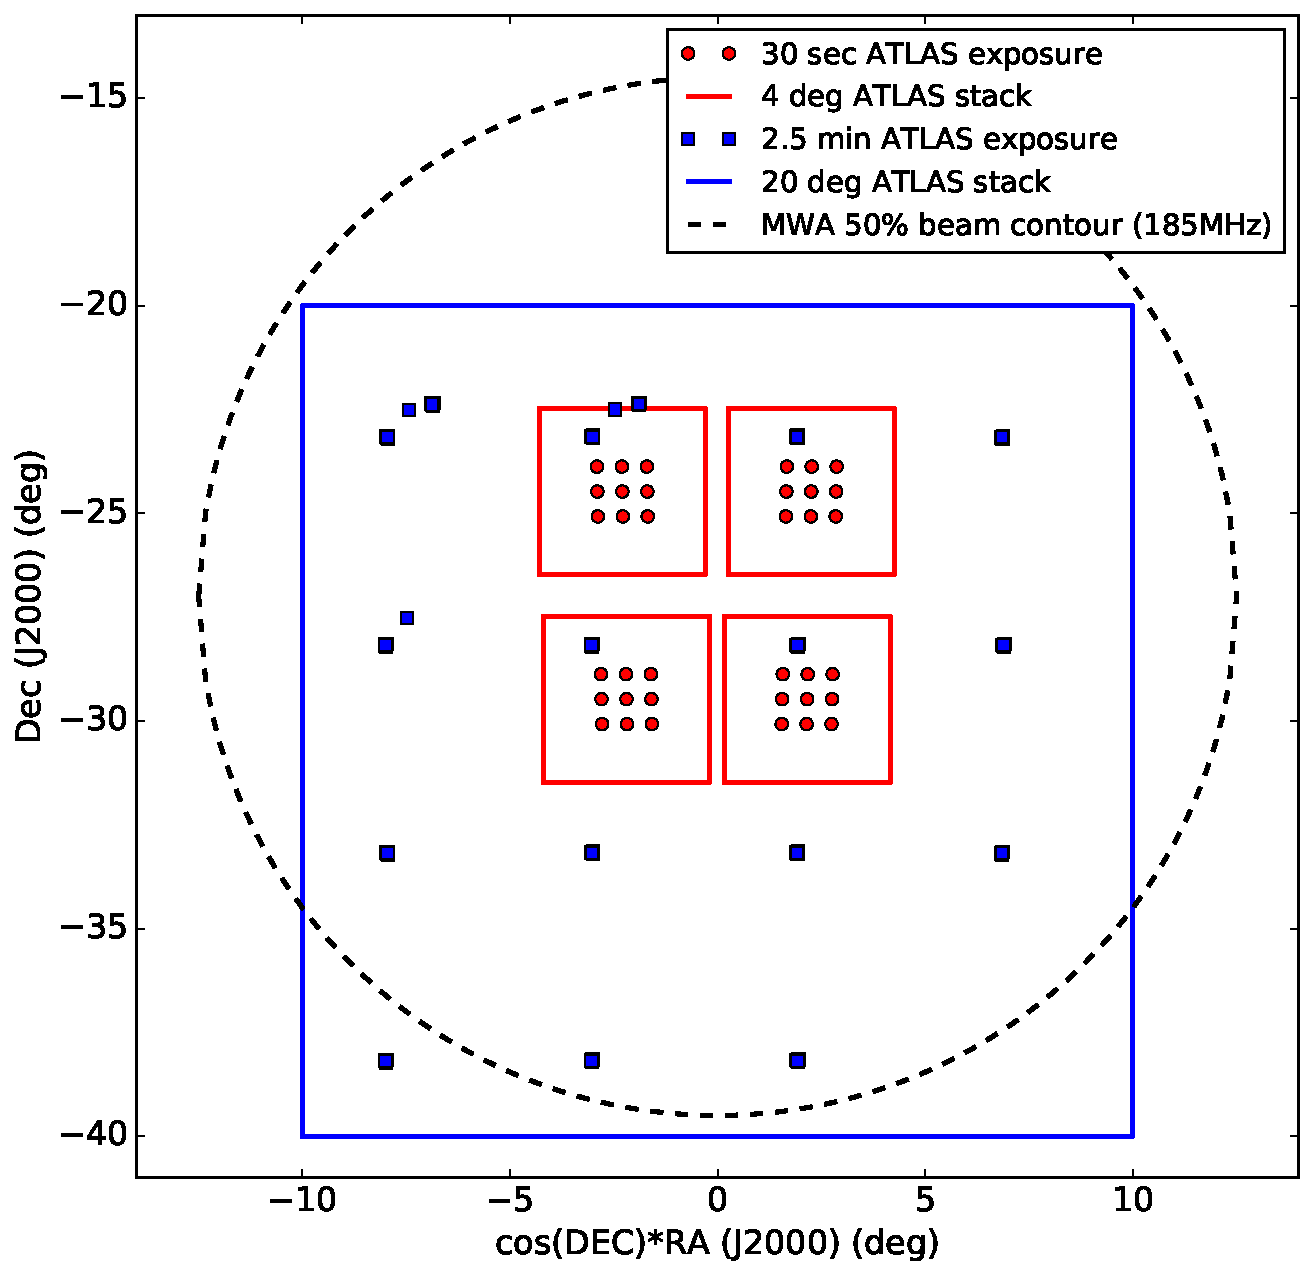
\includegraphics[width=3.3in]{images/survey_overview.pdf}
\caption{The MWA deep integration field (black dashed circle) is shown relative to our two ATLAS surveys. Blue markers show the observation centers of our wide ATLAS survey aimed at studying foregrounds, and the large blue square shows the stacked image. Red circle markers show observation centers for our slightly deeper survey, and red squares show the four stacked images we generate. Note that the ATLAS field of view is 5.5$^\circ$.}
\label{fig:surveyoverview}
\end{figure}

ATLAS is a 0.5\,m (f/2.0) telescope \citep{tonry11} in Hawaii designed to perform a wide field sky survey for near earth asteroids. The detector is a 10,500 $\times$10,500 STA-1600 CCD array, with a pixel scale of 1.86'', with an overall field of view of $5.5^\circ$. We observe in the \textit{i} band centered at 810\,nm with full width at half max 150\,nm, corresponding to $z=$5.1--6.3. While this redshift range doesn't exactly match that of our radio observations, it overlaps sufficiently for our purpose of characterizing the effects of noise foregrounds in 21cm--IR cross correlation experiments, and setting the first limits on the cross spectrum of residual foregrounds. 

ASK BRIAN TO WRITE A FEW SENTENCES ABOUT THE ATLAS CALIBRATION AND IMAGING PIPELINE

We perform two separate observing campaigns, which we illustrate in Fig. \ref{fig:surveyoverview}. We first perform a wide survey to best characterize bright foregrounds. We raster scan a roughly $20^\circ\times20^\circ$ grid with $5^\circ$ spacing over the MWA field (dashed black circle), integrating for 2.5\,min at each pointing (blue square markers). The observations are conducted between 2016/09/07 22:00  and 2016/09/08 00:50 Hawaii-Aleutian Standard Time, when the moon was 36\% illuminated. We then use {\tt swarp}\footnote{\ULurl{http://www.astromatic.net/software/swarp}} \citep{swarp} to stack all these frames over $20^\circ$ orthographic field centered on (RA,Dec) = $(0^\circ,-30^\circ)$ (blue square) with 1.86'' resolution, using the default background subtraction settings to mitigate temporal and spatial background variation. 

% moon phase calculator: http://www.moonpage.com/index.html?go=T&auto_dst=T&tzone=ut&m=9&d=8&y=2016&hour=0&min=51&sec=45

Our second campaign is a slightly deeper survey designed to better mitigate airglow fluctuations and CCD systematics for the purpose of studying faint foregrounds. We select four 5 deg fields positioned around the MWA beam peak for best cross correlation precision: (RA,Dec) = $(-2.5^\circ, -24.5^\circ)$, $(2.5^\circ, -24.5^\circ)$, $(-2.5^\circ, -29.5^\circ)$, $(2.5^\circ, -29.5^\circ)$ (J2000). We raster scan a $3\times3$ grid of 30\,sec observations within each field (red circle markers) intended to mitigate slight amplifier non-uniformities across the CCD array. The observations were conducted on 2016/11/02 between 21:47 and 23:11 Hawaii-Aleutian Standard Time, when the moon was 5\% illuminated. 

We stack the frames in each of the four deep fields using {\tt swarp} over only the central $4^\circ\times 4^\circ$ region over which all nine 30\,sec frames overlap (red squares). Otherwise slight background discontinuities would be introduced by the different temporal coverage of different regions of the stack. In this stacking, we disable background subtraction for the purpose of studying later on the effects of airglow-induced diffuse backgrounds.

\section{Point source foregrounds}

\subsection{Catalogs}
\label{sec:catalogs}

To characterize the bright sources relevant to broad band  21\,cm--Ly$\alpha$ and  21\,cm--H$\alpha$ intensity mapping correlation measurements we calculate the correlations between catalogs at 185\,MHz, 850\,nm, and 4.5\,um as a function of mask depth. These bands correspond roughly to 21\,cm, Ly$\alpha$, and H$\alpha$ at $z\sim6-7$, respectively. 

\begin{figure*}[t]
\centering
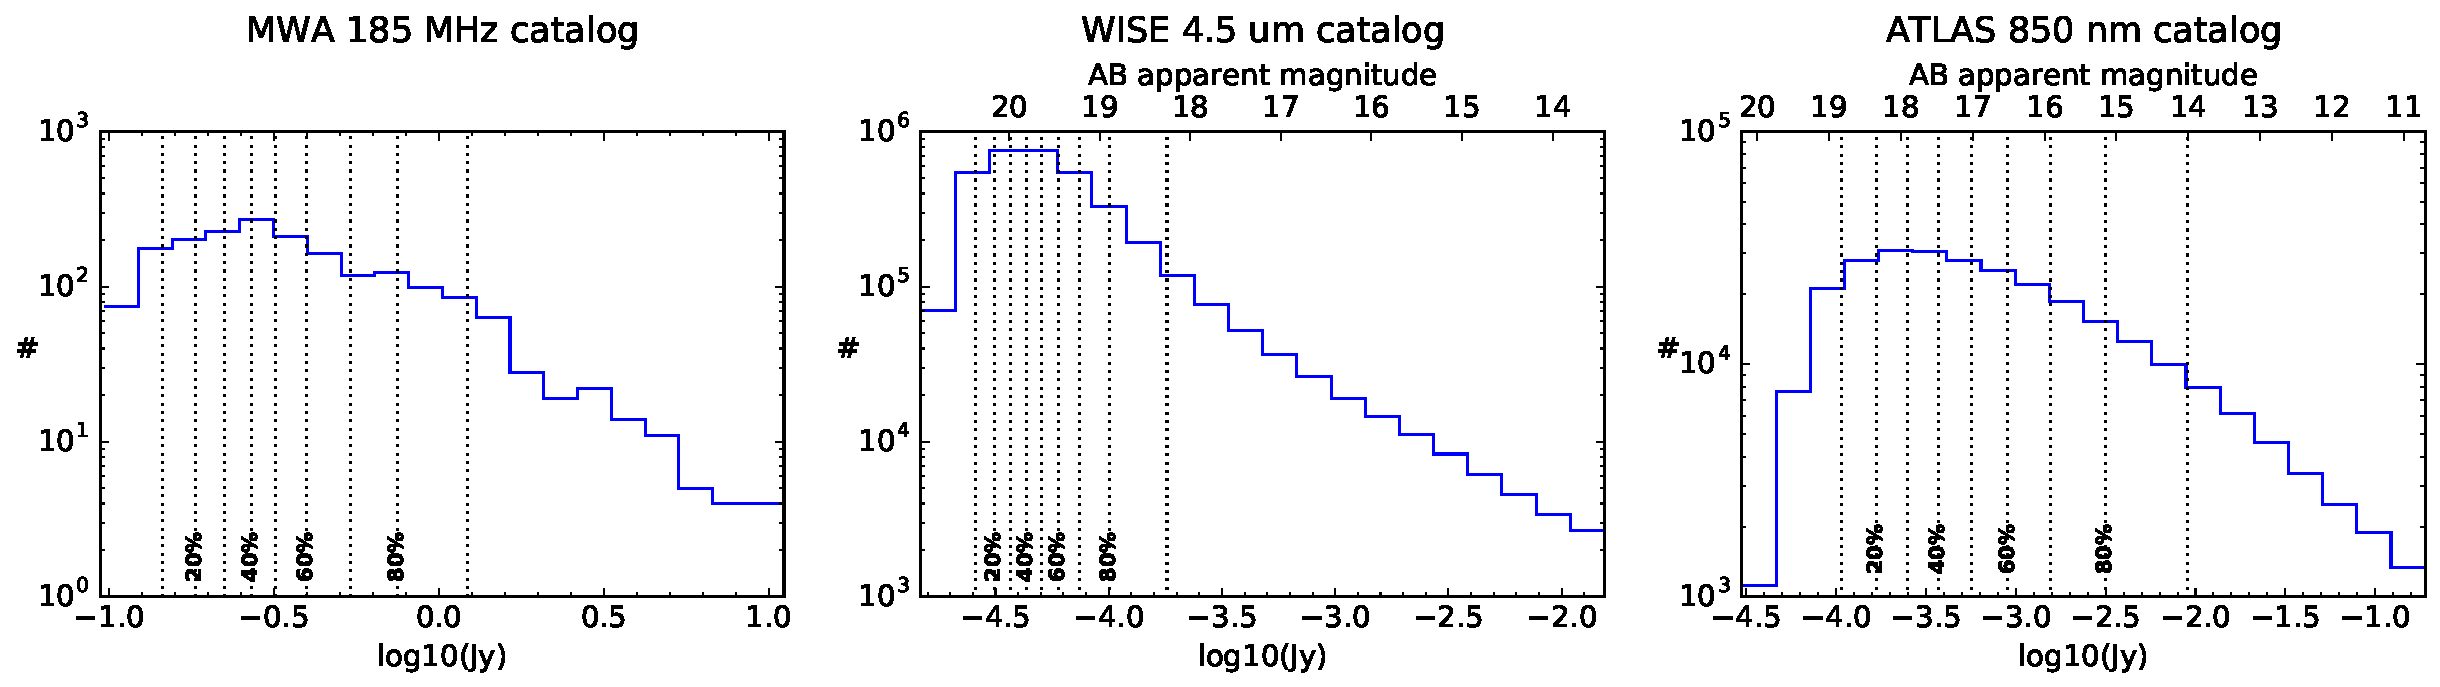
\includegraphics[width=6.5in]{images/catalog_histograms.pdf}
\caption{Histogram of source fluxes in the 185\,MHz catalog (left), the 4.5\,um catalog (center), and the 850\,nm catalog (right). The catalogs are complete to roughly 300\,mJy, 0.05\,mJy, and 0.3\,mJy respectively.}
\label{fig:cataloghistograms}
\end{figure*}

We use the 185\,MHz catalog reduced from deep observations of the MWA field depicted in Fig. \ref{fig:surveyoverview} by \citep{PattiCatalog1}. Fig. \ref{fig:cataloghistograms}) (left panel) shows a histogram of source fluxes in this field. The survey depth varies somewhat over the MWA field due to the varying primary beam, though within the full-width-at-half-max it is complete to roughly 300\,mJy. Note that the completeness varies across the field, with fewer fainter sources detected away from the pointing center as the beam weakens. MWA astrometry is at the 2'--3' level due to the MWA's short baselines, though \citep{PattiCatalog1} cross-match with higher frequency catalogs to achieve order 10'' astrometry. 

We use the W2 band of ALLWISE \citep{Wright2010,allwise} as our 4.5\,um catalog. We download the list of sources within the MWA field using the All Sky Search on the NASA/IPAC Infrared Science Archive\footnote{\ULurl{http://irsa.ipac.caltech.edu}}, and plot the histogram of source fluxes in Fig. \ref{fig:cataloghistograms}) (center panel). This ALLWISE band is specified to be 95\% complete to 88\,$\mu$Jy (15.7 AB mag), though it has slight sky coverage non-uniformities due to satellite coverage.

Lastly, we run SExtractor\footnote{\ULurl{http://www.astromatic.net/software/sextractor}} \citep{sextractor} on our wide $20^\circ$ wide ATLAS composite image to generate an 850\,nm catalog. We allow local background bias and noise estimation, set pixel saturation at 20,000 counts to avoid artifacts, and use the {\tt AUTO} aperture profile. We extract sources down to $3\sigma$ above the background, in order to achieve the most complete point source mask. Given that our ATLAS observations have been calibrated and imaged through a preliminary pipeline, we cross match these sources with sources closer than 1'' in the AAVSO Photometric All Sky Survey\footnote{\ULurl{https://www.aavso.org/download-apass-data}} \citep{apass}, finding matches $\sim10\%$ of the time. Fig. \ref{fig:ATLASvsAPASS} (top) shows a 2D histogram of APASS versus ATLAS magnitude as a function of ATLAS magnitude. We fit a gaussian to the relative magnitude for sources brighter than 13 mag, and find that out roughly calibrated ATLAS sources are too bright by $0.279\pm0.003$\,mag. Applying this correction, we plot a histogram of ATLAS source fluxes in Fig. \ref{fig:cataloghistograms}) (right panel), finding that our survey is complete to roughly 1\,mJy.

\begin{figure}[t]
\centering
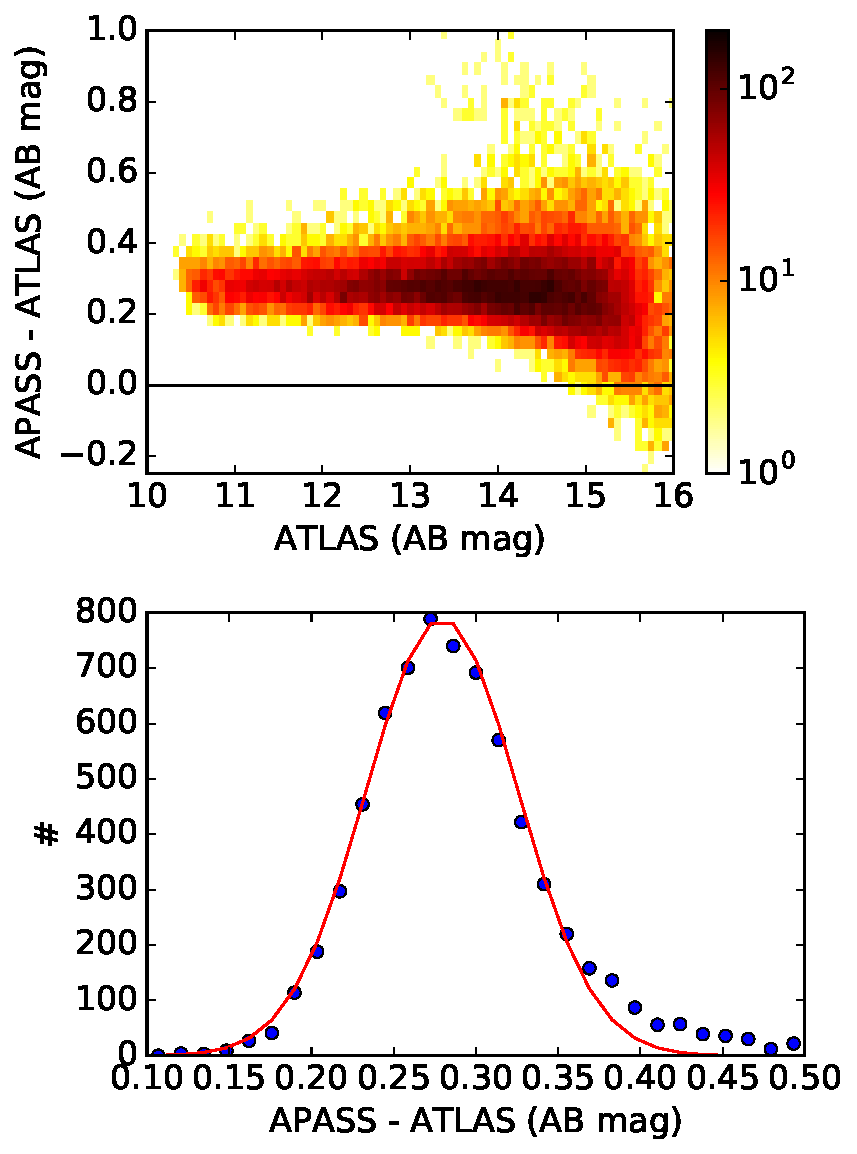
\includegraphics[width=2.75in]{images/ATLAS_vs_APASS_cal.pdf}
\caption{To improve the rough initial ATLAS calibration, we cross match ATLAS sources with those from APASS, and plot a 2D histogram (top) of the relative magnitude as a function of ATLAS magnitude, then fit a gaussian to the magnitude offset for sources brighter than 13\,mag. We find that our roughly calibrated ATLAS sources are too bright by $0.279\pm0.003$\,mag.}
\label{fig:ATLASvsAPASS}
\end{figure}

We find the catalog is complete to roughly a mJy (right panel in Fig. \ref{fig:cataloghistograms}). 



\subsection{Catalog radio--infrared flux correlations}
\label{sec:catcorrelations}

Having prepared catalogs of point source foregrounds in our three bands, we proceed to study how they manifest in intensity mapping correlation experiments. Traditionally, radio/infrared correlations have been studied by cross matching high frequency radio detections with infrared sources coincident within a few arcseconds, thenn plotting radio versus infrared luminosity. Such studies have revealed the well known radio--far infrared correlation thought to be due to massive star formation \citep[e.g.][]{helou85,dejong85,yun01,xu94}. Massive stars blow out ionized bubbles, generating radio free-free emission correlated with the ionizing flux. Some fraction of these high energy photons are absorbed by dust clouds and reprocessed into far-infrared \citep{xu94}. At radio frequencies lower than $\sim10$\,GHz, synchrotron dominates over free-free emission, and the correlation is thought to arise from the acceleration of cosmic ray electrons in these stars' supernovae. 

Our approach is different. For all the advantages of broad band intensity mapping, sources cannot be localized to specific redshifts, meaning that it is foreground fluxes, not luminosities, whose correlations are of interest. Of course compact foregrounds may be masked or subtracted to some residual level, but any correlation of these residual foreground fluxes could mask the cosmological correlation. We begin in this section by analyzing foreground fluxes as a function of masking depth, and in the next section turn to the foregrounds in residual images below the detection limit of these catalogs. A last comment on our approach is that though searching for radio--infrared correlations on a source-by-source level would be valuable cross check, we lack the radio astrometry to do so\footnote{In their cross matching study of GHz radio sources with optical detections, \citep{mcmahon02} find that 99\% of cross-matches within 10'' of each other (see their Fig. 8), of order the positional accuracy quoted by \citet{PattiCatalog1}.}. 

\begin{figure*}[h]
\centering
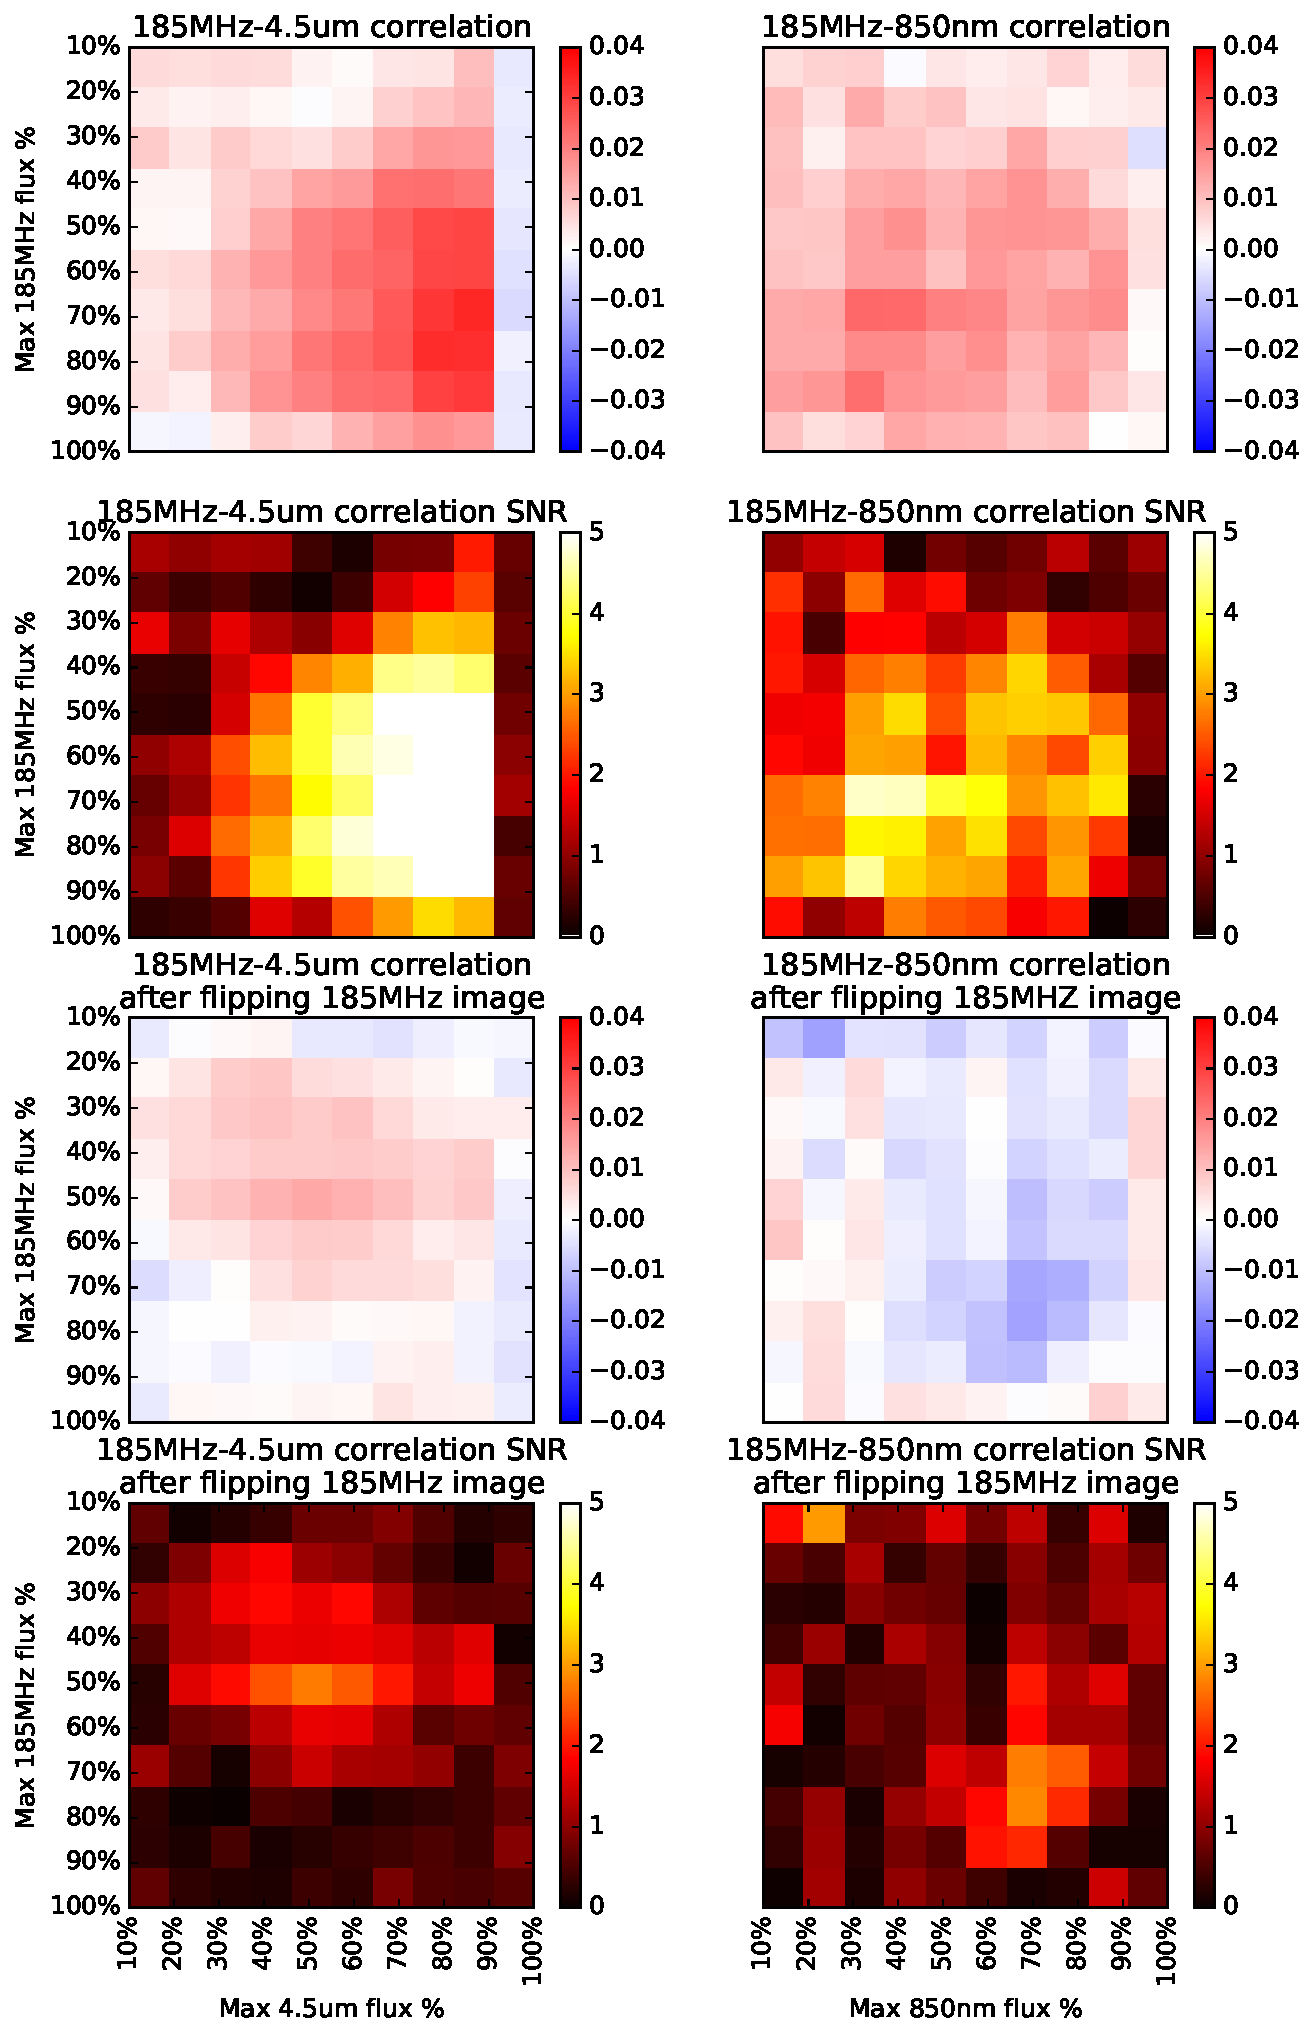
\includegraphics[width=5.5in]{images/source_correlation_grids_and_snrs.pdf}
\caption{Image space correlation coefficient between 185\,MHz and 4.5\,$\mu$m sources (top left), and 185\,MHz and 850\,nm sources (top right), both as a function of radio and infrared flux cuts. Excluding the top 10\% of sources (down to $10^{-3.5}$\,Jy at 4.5\,$\mu$m and $10^{-2}$\,Jy at 850\,nm is a good proxy for removing the stars, below which we observe a 5\% 185\,MHz--4.5\,$\mu$m correlation and a marginal percent level 185\,MHz--850\,nm correlation. In the second row we calculate the SNR in each bin, noting that neighboring bins are somewhat correlated. The bottom two rows show the correlations and SNRs after flipping the 185\,MHZ image in the calculation calculation, giving an independent estimate of the noise.}
\label{fig:correlationsandSNRs}
\end{figure*}

We begin by gridding all three catalog fluxes in Jy to the $20^\circ\times20^\circ$ grid centered at (RA,Dec) = $(0, -30^\circ)$ depicted in Fig. \ref{fig:surveyoverview}, and calculating the zero delay correlations between the images as
\begin{equation}
\label{eqn:imagecorrdef}
	c = \frac{\langle I_\rad I_\IR\rangle-\langle I_\rad\rangle\langle I_\IR\rangle}{\sqrt{(\langle I_\rad^2\rangle -\langle I_\rad\rangle^2)(\langle I_\IR^2\rangle -\langle I_\IR\rangle^2)}}
\end{equation}
where the uncertainty due to sample variance is approximately $dc=N_\text{pix}^{-1/2}$, where $N_\text{pix}$ is the total number of pixels in the image. Between MWA and WISE catalogs we find $c=-0.003\pm0.005$ and between MWA and ATLAS catalogs we find $c=0.001\pm0.005$. Both are consistent with zero, as expected, as the brightest sources in both infrared catalogs are likely stars, whose radio emission is vanishingly small. As an experiment, we recalculate these correlations after excluding the brightest 10\% of sources in all three catalogs, effectively masking down to $10^{-3.75}$\,Jy at 4.5\,$\mu$m and $10^{-2}$\,Jy at 850\,nm, and find $c_\text{MWA--WISE}=0.031\pm0.005$ and $c_\text{MWA--ATLAS}=0.0086\pm0.005$. The former is a $6\sigma$ detection, and merits some investigation. How does this apparent correlation depend on the flux cut? What is it due to? And what does it mean for broad band correlation experiments? Further, does the MWA--ATLAS correlation remain consistent with zero at stricter flux cuts?

To begin to answer these questions, we plot in Fig. \ref{fig:correlationsandSNRs} the 185\,MHz--4.5\,$\mu$m correlation (top left) and 185\,MHz--850\,nm correlation (top right) as a function of the maximum flux percentile allowed in the data (masking depth). We plot the SNRs of these correlation measurements, taking the noise to be $1/\sqrt{N_\text{pix}}$ as described above, in the next row. Note that adjacent cells in the correlation matrix plots are somewhat correlated, so a consistent positive sign is not in and of itself evidence of significance. We assess significance by comparing of each correlation measurement individually with the expected noise (the SNR), as well as by checking that the correlation vanishes when the 185\,MHz image is flipped (bottom two rows).

The 185\,MHz and 4.5\,$\mu$m catalogs exhibit a positive correlation peaking at $0.0332\pm0.005$ after masking infrared sources down to 10$^{-4}$\,Jy (18.9\,mag) and radio sources down to 1\,Jy, and remains significant down to the completeness limits of these catalogs. There is no significant correlation detection after flipping the 185\,MHz image, indicating this detection is not an artifact of the analysis. The 185\,MHz and 850\,nm catalogs exhibit a marginal $3\sigma$ correlation after masking infrared sources down to 10$^{-3}$\,Jy (16.4\,mag) and radio sources down to 0.3\,Jy, though it does not appear significant in comparison to the level of correlation noise in the flipped image.

To understand these findings, we begin by digging deeper into the 4.5\,$\mu$m catalog. We select the subset of sources detected in the WISE 3.4\,$\mu$m, 4.5\,$\mu$m, and 12\,$\mu$m bands and plot them (Fig. \ref{fig:wisecolorcolor}, left panel) in the $W_{23}\equiv$[4.6\,$\mu$m] -- [12\,$\mu$m] versus $W_{12}\equiv$[3.4\,$\mu$m] -- [4.6\,$\mu$m] color-color space used by \citet{Wright2010} to illustrate the separation different types of sources. \citet{nikutta14} study more quantitatively how these different sources separate in this color space, finding that stars separate clearly from all other sources in the region $W{12}=-0.04\pm0.03$, $W_{23}=0.05\pm0.04$ (1$\sigma$). In the right panel, we plot the faintest 90\% of sources (fainter than 18.25 mags at 4.6\,$\mu$m) in the same color-color space and observe this cut effectively cleanly excludes nearly all the stars. This explains why when masking this brightest 10\% earlier, we observed zero correlation with 185\,MHz sources, and why afterward the correlation suddenly emerges, after all, nearly all radio sources are non-stellar (i.e., extragalactic). 

\begin{figure*}[h]
\centering
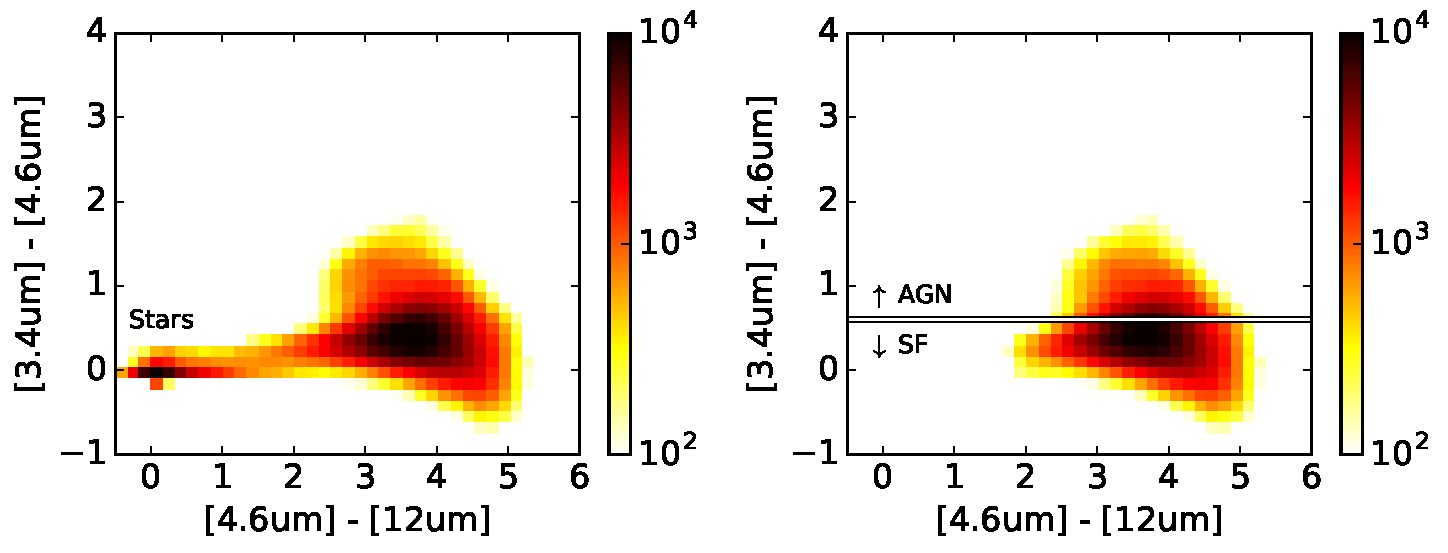
\includegraphics[width=6in]{images/wise_color_color_figure_max=1e-3_5Jy.pdf}
\caption{The ALLWISE sources are plotted in the color--color space of \citet{Wright2010} prior to any flux cuts (left panel), showing the stars near (0,0). Then after cutting out the brightest 10\% of sources (fainter than 18.25\, AB mag), the stars are cleanly removed. We roughly split the remaining sources into AGNs ($W_{12}>0.16$) and starburst galaxies (SF) ($W_{12}<0.16$) \citep{nikutta14,kurcz16}}.
\label{fig:wisecolorcolor}
\end{figure*}

To further probe which mid infrared sources are responsible for this correlation, we make a rough cut to separate quasars and active galactic nuclei (AGNs) ($W_{12}>0.16$) from starburst galaxies (SFs) ($W_{12}<0.16$) \citep{nikutta14,kurcz16}. In Fig. \ref{fig:wisexspec} we plot the power spectrum of 185\,MHz sources (left panel), the spectra of our AGN and SF cuts of 4.5\,$\mu$m sources (center panel), and the coherence (i.e., correlation coefficient versus $\ell$) of each of these cuts with the 185\,MHz catalog (right panel). The AGN subset exhibits no significant correlation with the 185\,MHz sources, while the SF cut exhibits a significant correlation rising from a few percent at $\ell\sim7000$ to 13\% at $\ell\sim300$. 

\begin{figure*}[h]
\centering
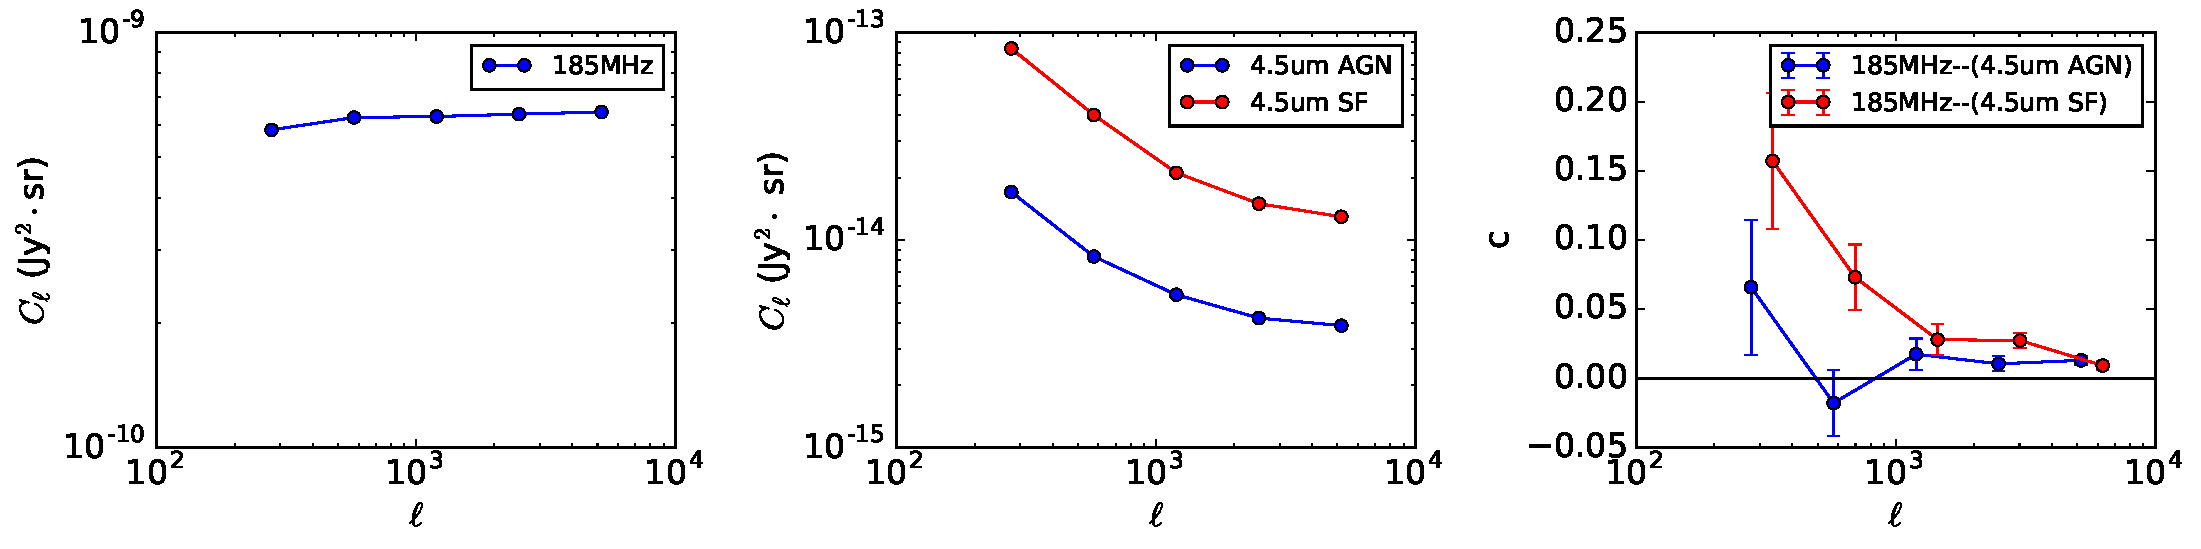
\includegraphics[width=7in]{images/mwa_wise_qsoagn_gal_xspec.pdf}
\caption{Power spectrum of 185\,MHz sources (left panel), 4.5\,$\mu$m sources (center panel), and coherence between 185\,MHz and 4.5\,$\mu$m sources (right panel). We roughly separate the 4.5\,$\mu$m sources into starforming galaxies (SF) and active galactic nuclei (AGN) as illustrated in Fig.  \ref{fig:wisecolorcolor}. We find that the 185\,MHz--4.5\,$\mu$m correlation observed in Fig. \ref{fig:correlationsandSNRs} holds only for the starforming galaxies in the infrared sample. }
\label{fig:wisexspec}
\end{figure*}

%argue that LRGs are negligible in terms of radio emission compared to LRGs

The fall of the correlation towards high $\ell$ is likely due in part to the MWA's 2' resolution at 185\,MHz, corresponding to a maximum $\ell$ of roughly 6000, and in part to the similar fall in the 4.5\,$\mu$m catalog power spectrum. Both the falling 4.5\,$\mu$m catalog power spectrum and the relatively flat 185\,MHz power spectrum are functions of the detailed properties of these surveys. \citet{tegmark02,dodelson02} show that the galaxy angular power spectrum $C_\ell$ is approximately equal to the 3D matter power spectrum $P(k(\ell))$ convolved with with a window function which depends on the redshift coverage and flux limit of the sample. The matter power spectrum is known to rise as $k^{1}$ for $k\lesssim0.02$\,h/Mpc, then falls as $k^{-3}$. Galaxy surveys typically probe the regime just above the turnover where the slope is transitioning from 0 to -3 \citep{tegmark02b}. In order to maximize its sensitivity to low surface EOR 21\,cm emission, the MWA was designed as a relatively compact array in comparison to higher resolution radio interferometers such as the Very Large Array. This low resolution makes the MWA catalog severely flux limited \citep{PattiCatalog1}, which in turn effectively masks many galaxies which would otherwise be seen. This large spatial mask translates into a wide fourier convolution kernel, explaining why the MWA catalog power spectrum is so flat. 

\subsection{Simulations of distance-induced flux correlation}

Let us now turn to addressing why the 4.5\,$\mu$mu SF sample is 5--15\% correlated with the 185\,MHz catalog, while the AGN sample is not. Of course some slight correlation is expected at some level as brighter AGN typically reside in more massive galaxies, which are typically brighter in stars as well (see, for instance, Fig. 1 in \citep{seymour07} or Fig. 4 in \citep{Willott03}) however \citet{mauch07} find no evidence of a radio/\textit{near}-infrared luminosity correlation anywhere near as strong as that between radio and \textit{far}-infrared emission.  However, as discussed above, broadband intensity mapping correlation experiments are affected not only by luminosity correlations between different bands, but flux correlations as well. We thus attempt to quantify to what extent fluxes in two different bands may appear correlated due to distance effects even when their intrinsic luminosities are completely independent of each other. By distance effects we refer to to the effect that more distant objects are generally weaker in all bands than nearer objects. 

We first make a few approximations to get intuition for the effect, and then simulate the effect as a function of stricter and stricter flux cuts due to deeper and deeper foreground masking. Consider a sky survey over a fixed field of view, and a set of objects with uncorrelated infrared and radio emission. By uncorrelated we mean that the infrared and radio luminosities are independent random variables determined by the infrared and radio luminosity functions, respectively. Assume that the objects are uniformly distributed in space out to $z\sim0.5$, and work in cartesian space for simplicity. We are interested in the effective correlation between radio and infrared fluxes in the same sky pixels, but let us approximate this by calculating the correlation between source fluxes in the two bands. Starting from Eqn. \ref{eqn:imagecorrdef}, we have
\begin{equation} % https://www.evernote.com/shard/s316/nl/2147483647/8270de10-6438-4d98-847a-a13e40ff9a14/
	c = \frac{\langle F_\rad F_\ir \rangle-\langle F_\rad\rangle\langle F_\ir\rangle}{\sqrt{(\langle F_\rad^2\rangle-\langle F_\rad\rangle^2)(\langle F_\ir^2\rangle-\langle F_\ir\rangle^2)}}
\end{equation}
Then writing this in terms of the radio and IR luminosities $F_i=L_i/4\pi d^2$ for $i=\rad,\ir$, we find
\begin{equation}
	c = \frac{\beta-1}{\sqrt{(\beta\alpha_\rad-1)(\beta\alpha_\ir-1)}}\approx(\alpha_\rad \alpha_\ir)^{-1/2}
\end{equation}
where $\beta\equiv\langle d^{-4}\rangle/\langle d^{-2}\rangle^2$ and $\alpha_i=\langle L_i^2\rangle/\langle L_i\rangle^2$.
For a survey of a fixed angular field of view, uniform spatial distribution of objects, and cartesian spacetime, the distribution of source distances $d$ grows as $d^2$, which gives 
\begin{equation}
	\beta\approx\frac{d_\maxtext^3-d_\mintext^3}{3d_\maxtext d_\mintext (d_\maxtext-d_\mintext)}
\end{equation}
We observe that the radio--infrared flux correlation for some type of objects is a function of their radio and infrared luminosity functions. In fact, we can see immediately that if the luminosity distributions are wide, their $\alpha$'s are large, and $c$ is small. Conversely, if the luminosity functions are narrow, then the distance to the sources plays a more significant role in determining their fluxes, and so $c$ is larger. 

\begin{figure*}[h]
\centering
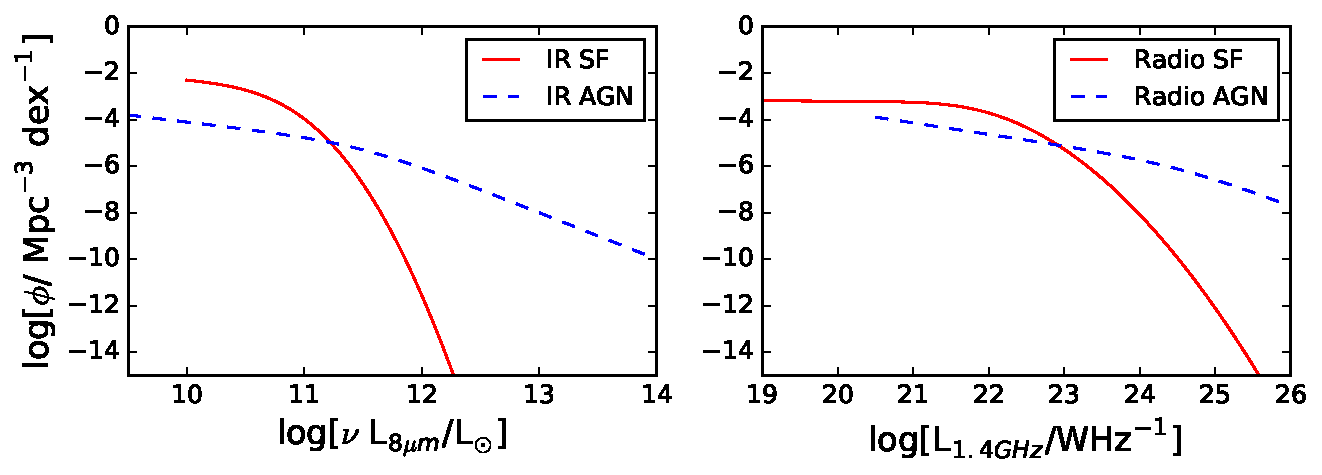
\includegraphics[width=6in]{images/sim_rad_ir_luminosity_functions.pdf}
\caption{AGN and SF luminosity functions at 8\,$\mu$m from \citet{fu10} (left panel) and at 1.4\,GHz from \citet{mauch07} (right panel).}
\label{fig:luminosityfunctions}
\end{figure*}

To quantify whether this effect can explain our measured radio--infrared correlation in SF galaxies and the lack of one in AGN, we use AGN and SF luminosity functions at 1.4\,GHz from \citet{mauch07} (Fig. \ref{fig:luminosityfunctions}, right panel) and at 8\,$\mu$m from \citet{fu10} (left panel). The former describe galaxies at $z<0.3$, while the latter describe galaxies at $z\sim0.6$. This analysis could be extended using proper redshift-dependent luminosity functions, possibly from simulations, though we find that despite these simplifications, our analysis suffices to explain our earlier measurements and we leave a more detailed study for future work. We use approximately the same range of luminosities used by \citet{mauch07} and \citet{fu10}, adjust the minimum luminosities slightly to achieve the same number density of AGN ($\sim0.0020$/Mpc$^3$) and SF ($\sim0.00011$/Mpc$^3$) in both radio and infrared surveys. In the end we find that our results are only slightly sensitive to these luminosity minima as their faint ends become less and less significant in real, flux-limited surveys. 

We pick fiducial survey parameters of $d_\mintext=20$\,Mpc and $z_\maxtext=0.75$\,Mpc, giving $\beta\approx54$.  Using the above luminosity functions, we find $\alpha_{\text{SF,IR}}=1.474$, $\alpha_{\text{SF,rad}}=14.56$, $\alpha_{\text{AGN,IR}}=22.97$, $\alpha_{\text{AGN,rad}}=257.5$. These values agree with qualitative observation that the AGN luminosity function is wider than the SF luminosity function in both radio and infrared bands (Fig. \ref{fig:luminosityfunctions}). These values give a predicted radio--infrared correlation of 0.21 for SF and 0.01 for AGN agreeing with our finding of a significant radio--infrared correlation for SF and near-zero correlation for AGN. The exact values deviate from our measurements for a number of reasons. The MWA and WISE catalogs are not matched in depth or redshift coverage, and thus don't survey an exactly overlapping set of radio and infrared sources. Further, real world luminosity functions can exhibit redshift evolution. Of course, our measurement above did not even split up the MWA catalog into separate AGN and SF subsets as such detailed characterization of low frequency radio foregrounds remains an active area of research. Lastly, the limited MWA resolution pushed the observed correlation with infrared images to zero at high-$\ell$, suppressing the overall correlation computed in image space from our simulation predicts.

\begin{figure*}[h]
\centering
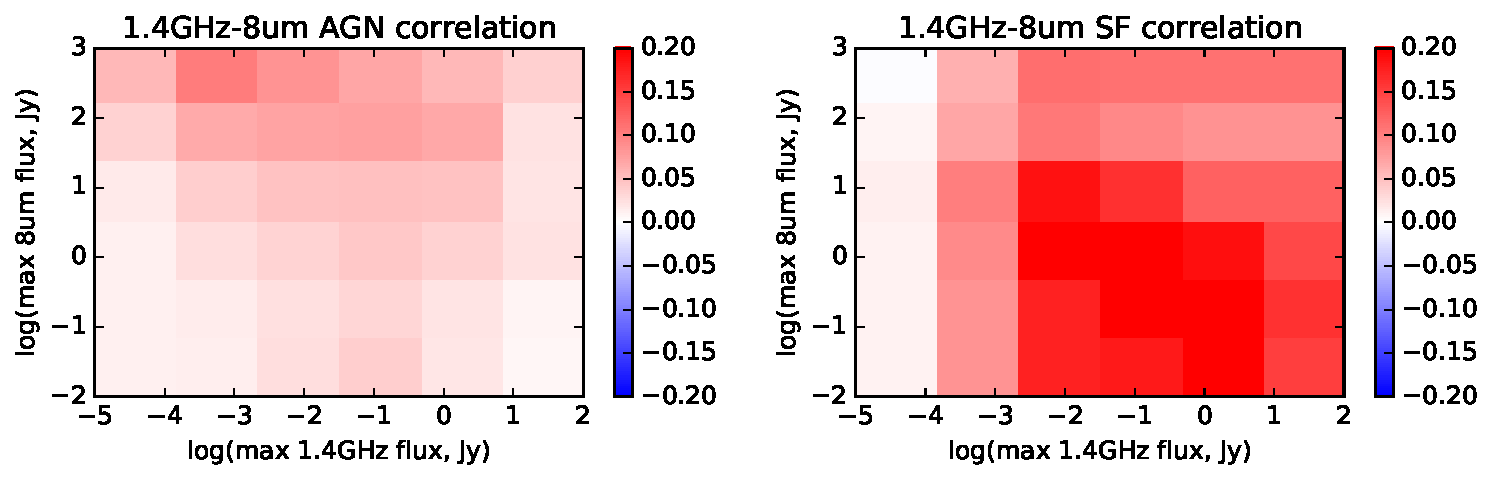
\includegraphics[width=6in]{images/sim_correlation_agn_and_sf.pdf}
\caption{Apparent correlation of radio and mid-infrared fluxes from a mock survey with uncorrelated radio and mid-infrared luminosities using the luminosity functions from Fig. \ref{fig:luminosityfunctions} for AGN and SF. Without any flux cuts (lower right corner of each plot) we observe a significant correlation between radio and mid-infrared fluxes for SF objects, and a near-zero correlation for AGN. This agrees with our measurements on real 185\,MHz and 4.5\,$\mu$m sources in Fig. \ref{fig:correlationsandSNRs}. As fainter and fainter objects are masked, we observe that the AGN correlation gradually strengthens, while the SF correlation weakens somewhat. We do not observe a monotonic trend, nor a general tendency towards zero as weaker and weaker sources are excluded. }
\label{fig:simagnlfcorrelations}
\end{figure*}

To what extent can this unwanted radio--infrared foreground correlation can be mitigated by masking the brightest sources. Using the luminosity functions presented above, we simulate radio and infrared surveys for each of AGN and SF. We begin by generating the mock radio catalogs of AGN and SF, choosing a poisson random number of each in each of 400 logarithmic luminosity bins. We distribute the objects uniformly over a volume $D_\maxtext=cz_\maxtext/H_0=$3212\,Mpc deep and $\theta_{\text{FOV}}D_\maxtext=$1121\,Mpc wide, then pick a random infrared luminosity for each radio object from the appropriate infrared luminosity function. Finally we plot in Fig. \ref{fig:simagnlfcorrelations}, along the lines of Fig. \ref{fig:correlationsandSNRs}, the predicted 1.4\,GHz--8\,$\mu$m correlation of our mock AGN and SF catalogs after masking down to a maximum radio and infrared flux. As we saw above, without any flux cut we find a roughly 20\% radio--infrared correlation for AGN and negligible correlation for SF. As we mask fainter and fainter sources, the AGN correlation generally increases to the 5--10\% level, while the SF correlation first increases, then decreases after masking down to 10$^{-4}$\,Jy. With increasing mask depth, these correlations do not change monotonically and they do not generally approach zero, and more detailed modeling of effective foreground flux correlations will be necessary in real world intensity mapping correlation experiments probing the EOR. In the next section we move beyond the bright sources and study the magnitudes and correlation properties of the residual radio and infrared foregrounds in our MWA and ATLAS observations.


\section{Residual foregrounds and cross spectrum limits}

In this section we characterize the power spectra and correlation properties of the residual 185\,MHz and 850\,nm foregrounds after subtraction and masking of the the bright sources identified by the surveys discussed in the previous section.

\subsection{Residual 21\,cm foregrounds}
\label{sec:res21fgs}

In this section we characterize the 185\,MHz foreground residuals in angular power spectrum measurements. We also quantify how much observation time is required to achieve the best foreground subtraction with an eye towards the large survey areas required to mitigate the sample variance noise due to uncorrelated radio and infrared foregrounds in cross spectrum analyses. In fact, while 21\,cm intensity mapping measurements in 3D are limited by radio thermal noise and demand order thousand hour integrations to reveal the cosmological signal \citep{beardsley13,PoberNextGen}, noise in broadband measurements is subdominant to foreground residuals after much shorter integration times. In fact, the $uv$ plane is essentially full after only 3 hours of rotation synthesis, and compounding days together serves only to increase signal to noise. 

The FHD outputs presented in Sec. \ref{sec:mwaobservations} are naturally weighted image space cubes of the raw data ($I_\text{nat}$), the model data ($I_\text{nat,mod}$), the synthesized beam ($I_w$) (i.e., the fourier transform of the $uv$ weights), and the primary beam. Each of these cubes has an \textit{odd} and \textit{even} version divided up at a 2\,sec cadence. We average all these cubes over frequency to make broad band images, then apply uniform weighting as in \citet{dillonneben} as
\begin{equation}
\label{eqn:uniformweighting}
I_\text{uni}(\vec{\theta}) = \frac{10^{-26}}{2k_B \lambda^2} \sum_{\vec{u}} \frac{\tilde{I}_\text{nat}(\vec{u})}{\tilde{I}_w(\vec{u})} e^{-2\pi i \vec{\theta}\cdot\vec{u}}d^2u
\end{equation}
where $\tilde{I}_i(\vec{u}) = \sum_{\vec{\theta}} I_i(\vec{\theta}) e^{2\pi i\vec{\theta}\cdot\vec{u}} d\Omega$ for $i=\text{nat},w$.

We then compute the angular power spectrum as
\begin{equation}
	C(\ell)=\frac{\sum_{\vec{\ell}}|\tilde{I}_\text{uni}(\vec{\ell})\tilde{I}_w(\vec{\ell})|^2}{\sum_{\vec{\ell}}|\tilde{I}_w(\vec{\ell})|^2}
\end{equation}
summing over all the $\vec{\ell}$ values in each $\ell$ bin. Note that $\ell=2\pi u$.  We estimate the thermal noise power spectrum by computing the power spectrum as above but using the odd minus even difference cube which contains only thermal noise.

\begin{figure}[h]
\centering
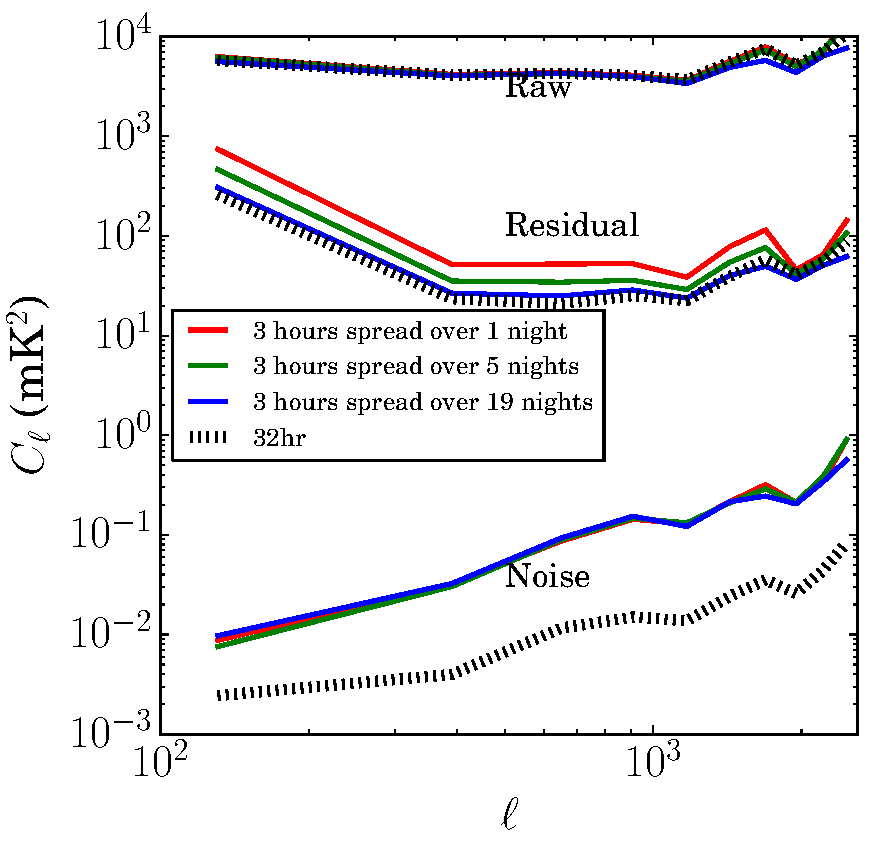
\includegraphics[width=3.5in]{images/res_pspec_of_100_obsids_with_diff_spacings_6amin.pdf}
\caption{Raw, residual (post foreground subtraction), and noise power spectra of 185\,MHz broad band images. We compare the 32\,hour deep integration of \citet{beardsley16} to 3\,hour integrations spaced over 1, 5, and 19 nights. The $uv$ plane is nearly filled after only 3\,hours, yet we find that spacing these $\sim100$ two-minute integrations over more and more independent nights reduces the foreground residuals by a factor of up to $\sim4$ in power. This bodes well for 21\,cm--infrared broad band correlation experiments as we will find later that a very wide survey is essential to average down the sample variance noise in uncorrelated radio and infrared foregrounds.}
\label{fig:respspecspacingsstudy}
\end{figure}

We plot in Fig. \ref{fig:respspecspacingsstudy} the power spectra of the raw, residual (post foreground subtraction), and noise images up to $\ell=2600$, corresponding to a maximum baseline length of $\sim$700\,m. Beyond this, the $uv$ coverage becomes quite sparse, introducing artifacts in the application of gridding and uniform weighting, though a more sophisticated analysis could likely use these long baselines. We compare the power spectra of the deep 32 hour integration of \citet{beardsley16} (black dashed) to those of 3 hour integrations spread over 1 (red), 5 (green), and 19 (blue) nights. Each of three three datasets consists of $\sim$100 two-minute integrations with a minimum spacing of 0, 5, and 24 minutes, all with occasional few-day gaps due to observing constraints and quality cuts. 

We find that all four sets have nearly identical raw power spectra. However, the residual power spectrum decreases as the 3 hours are spread over more and more nights until it reaches the level of the deep 32 hour integration, a factor of $\sim4$ lower in power than that of the single night analysis. These findings are consistent with ionosphere-related errors, e.g., in sky model calibration, where source position errors due to the ionosphere may require many independent nights to average down. Thus while we use the 32 hour integration for convenience in this analysis, it is by no means necessary to use such a deep integration in a broad band analysis, especially when we will find later that survey speed is essential for such broad band correlation experiments. Note that as expected, the thermal noise of the deep integration is a factor of $\sim10$ in power below that of the 3\,hour integrations, which are themselves at least a factor of $\sim100$ below the foreground residuals in these broad band images.

\subsection{Residual IR foregrounds}
\label{sec:resirfg}

We proceed to generate foreground-subtracted 850\,nm images of the four deep ATLAS integration fields shown in Fig. \ref{fig:surveyoverview}. Each of these fields is a stack of 9 30\,sec exposures with 5$^\circ$ field of view, dithered such that the overlap is a $\sim4^\circ$ region. By confining ourselves to this overlap region, we avoid the background discontinuities which affect many nominally wide field infrared image datasets whose mosaicing introduces significant background patchiness. 

Our approach is to mask each image at 1.86'' resolution, then coarse grid down to $3.5'$, of order the resolution of the MWA, taking each coarse pixel's value as the average of all unmasked fine pixels within it. If fewer than 10\% of its fine pixels remain unmasked, we consider the whole coarse pixel masked to avoid introducing too much noise variation over coarse pixels. We apply the high resolution source masking in the following four stages, which we illustrate in Fig. \ref{fig:bigfgmaskingstudy} for the ATLAS field centered at (RA,Dec)$=2.74^\circ, -24.79^\circ$) (the top right red box in Fig. \ref{fig:surveyoverview}). Each row shows the result of an additional masking stage, as outlined below. The left column shows a typical 9' field to illustrate the masking up close; the center column shows the coarse binned image with $3.5'$ resolution; and the right column shows the FFT of the center image (plotted as $\log[\Delta(\vec{\ell})/(\text{kJy/sr})]$) in order to identify detector systematics. 

\begin{figure*}[h]
\centering
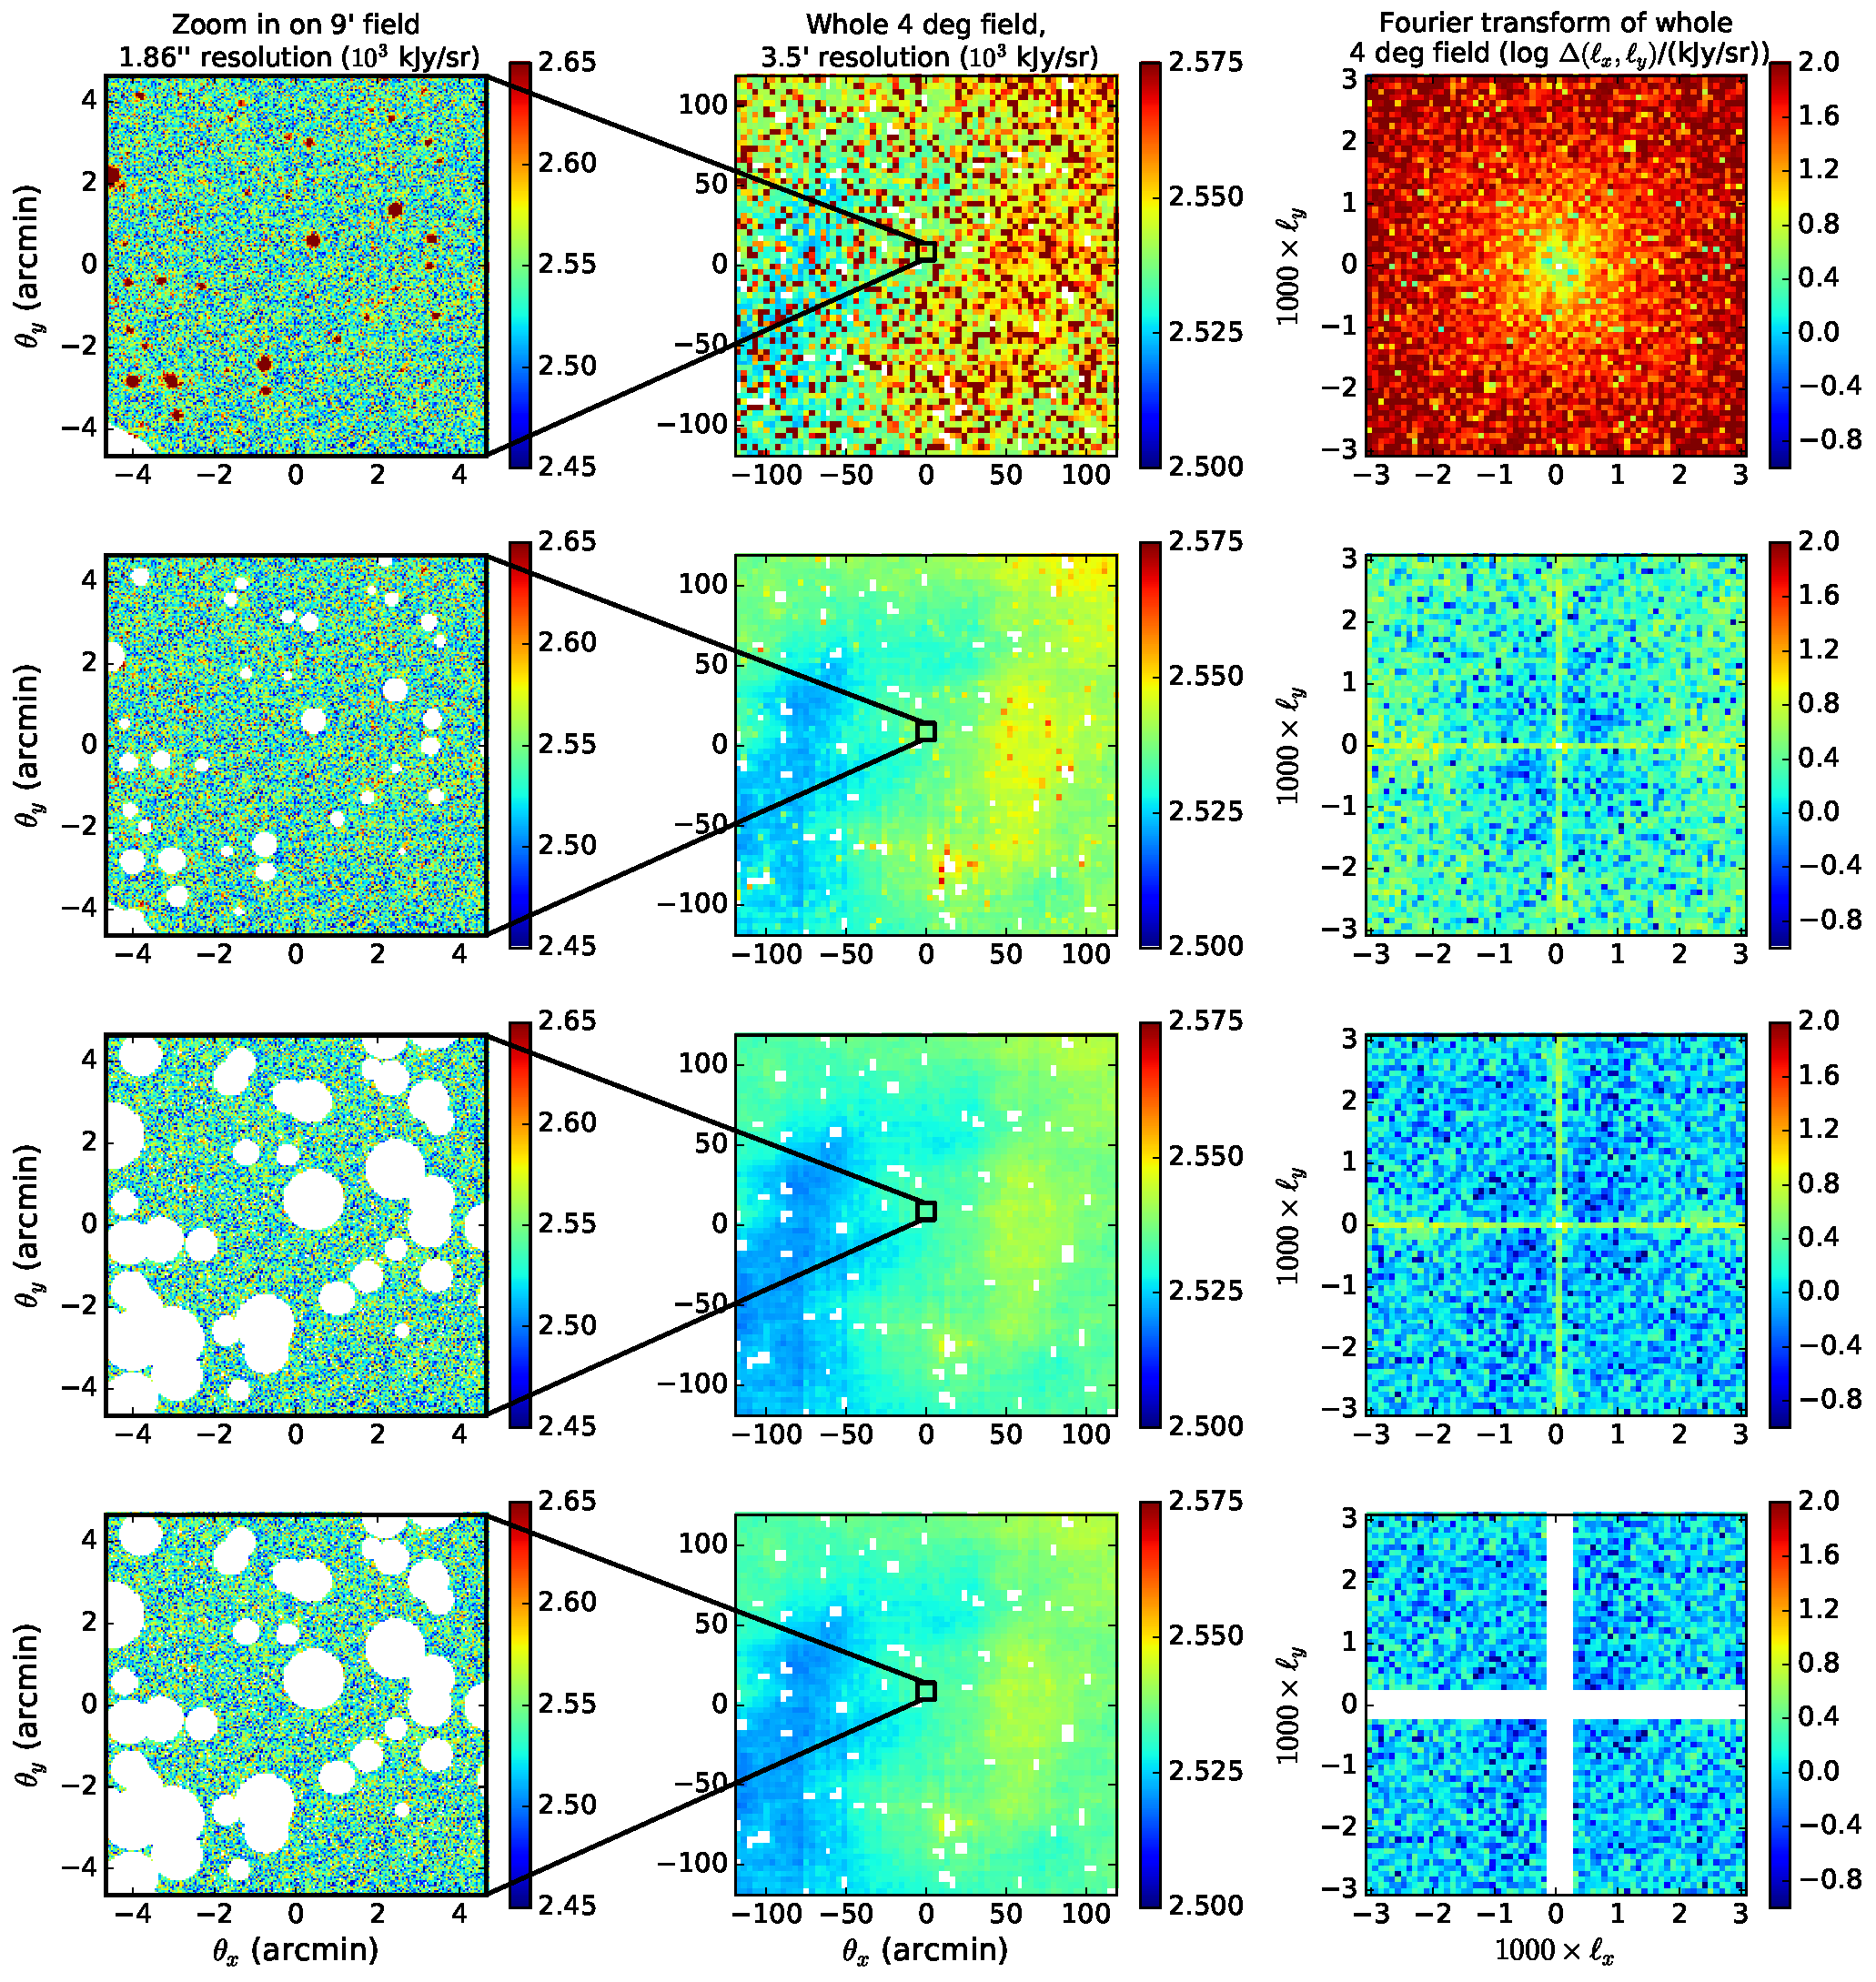
\includegraphics[width=7in]{images/big_foreground_masking_study_2_magoffset=20_56+0_274.pdf}
\caption{This shows illustrates the four stages of foreground removal we perform on ATLAS images, as detailed in Sec. \ref{sec:resirfg}. We apply this process to all four $4^\circ$ deep ATLAS fields shown in Fig. \ref{fig:surveyoverview}, but here use the one centered at (RA,Dec)$=2.74^\circ, -24.79^\circ$) for illustration. The first shows the results of masking 4' around all nearly saturated regions; the second row shows the results of masking out to $5\sigma$; the third row shows the results after masking out to $12\sigma$ and all pixels above 70\,kJy/sr over the background, and the last row shows the results after masking the nearly horizontal or vertical fourier modes. In each row, we show a typical 9' field at 1.86'' resolution (left), the whole $4^\circ$ field after coarse gridding to $3.5'$ (center), and the FFT of the coarse gridded field to highlight systematics (right). Note that the left and center panels of the bottom row are identical to those in the row above it, illustrating that the image space mask is the same, only the fourier mask is different.}
\label{fig:bigfgmaskingstudy}
\end{figure*}

\begin{enumerate}
	\item \textbf{Mask saturated regions.} (Fig. \ref{fig:bigfgmaskingstudy}, row 1) Nearly saturated pixels are associated with nearby bright stars which would dominate fluctuation measurements, we thus mask 4' around all pixels within 30\% of saturation (white regions in left and center columns). This wide mask removes the broad wings of the PSF revealed by these extremely bright sources. On average over our fields, 92\% of fine pixels remain unmasked after this step, and 96\% of coarse pixels remain.
	\item \textbf{Mask sources to 5$\sigma$.} (Fig. \ref{fig:bigfgmaskingstudy}, row 2) We mask circular regions with radius equal to five times the profile RMS along the minor axis of each source as measured by SExtractor (see Sec. \ref{sec:catalogs}). The reason we use the minor axis RMS is that vertical charge leakage in the CCD array results in unrealistically large major axis RMS measurements for bright sources. After this stage $\sim87$\% of fine pixels remain unmasked, and the fraction of coarse pixels remaining is unaffected.
	\item \textbf{Mask sources to $12\sigma$ and other emission above 70\,kJy/sr over the background.} (Fig. \ref{fig:bigfgmaskingstudy}, row 3) We use a larger masking radius to remove the PSF wings around the 5$\sigma$ source masks. We also determine that the vertical CCD charge leakage can be isolated by looking for emission brighter that 70\,kJy over the background, and that it can be flagged without cutting into the shot noise between sources. 58\% of fine pixels remain unmasked after this step, and again the fraction of coarse pixels remaining is unaffected.
	\item \textbf{Mask horizontal and vertical fourier modes.} (Fig. \ref{fig:bigfgmaskingstudy}, row 4) The previous two stages revealed detector artifacts within $\Delta\ell \sim100$ of $\ell_x=0$ and $\ell_y=0$. These compact fourier systematics correspond to slight horizontal and vertical discontinuities in the center image due to imperfect gain matching between 16 different detector amplifiers which process different rectangular regions of the CCD array. We conservatively mask fourier modes with $|\ell_x|<200$ or $|\ell_y|<200$ to eliminate this effect.
\end{enumerate}

Note that these 850\,nm deep observations were recorded during near new moon conditions, and we find that the mean air glow in source-free regions is $\sim3\times10^3$ kJy/sr, of order 19 AB mag/arcsec$^2$. \citet{sullivan12} measure a 1020\,nm continuum air glow brightness (i.e., after spectrally masking the OH lines) of $20\pm0.5$ AB mag/asec$^2$ far away from the moon. 

We proceed to characterize the residual infrared fluctuations in power spectrum space, using the optimal quadratic estimator to properly account for the masking of coarse pixels. This estimator was introduced to astronomy by \citet{Maxpowerspeclossless} to recover CMB power spectra from maps with arbitrary survey geometries and noise properties, and has recently been revived for 3D power spectrum analysis of 21\,cm data by \citet{X13, dillonneben, LT11, DillonFast, ali15}. We employ this estimator in a manner more similar to the original CMB case, using it to account for pixel masking in broad band power spectrum estimation. We briefly summarize the estimator here, and refer to \citet{X13} for a more detailed description.

We label the normalized estimator of the power in bin $\alpha$ as $p_\alpha$, related to the unnormalized estimator $q_\alpha$ as $\mathbf{p} = \Mb \mathbf{q}$. Bold lower-case letters are vectors, while bold upper-case letters are matrices. The unnormalized estimator is given by
\begin{equation}
q_\alpha = \frac{1}{2}(\xb-\langle\xb\rangle)^t \Cb^{-1} \Cb_{,\alpha}\Cb^{-1}(\xb-\langle\xb\rangle)
\end{equation}
where $\xb$ is a column vector containing all $N_\text{pix}$ pixel measurements, $\Cb$ is the pixel-pixel covariance matrix, and $\Cb_{,\alpha}\equiv d\Cb/dp_\alpha$ is the derivative of the covariance with respect to the power in bin $\alpha$. Note that $\Cb_{,\alpha} = \Ab^\dagger\Ab$, where $\Ab$ is a $N_\alpha\times N_\text{pix}$ with elements $A_{ij}=\exp(i\vec{\theta}_j\cdot\vec{\ell}_i)$. Here $\vec{\ell}_j$ refers to the $j$'th out of $N_\alpha$ $\vec{\ell}$ modes in bin $\alpha$. Note that $^t$ denotes a transpose, and $^\dagger$ donates conjugate transpose.

The matrix of window functions (i.e., horizontal error bars) of the band powers $p_\alpha$, defined such that $\pb_\text{estimated}=\Wb\pb_\text{true}$ is given by $\Wb=\Mb\Fb$, where $\Fb$ is the Fisher matrix and $\Mb$ is an arbitrary invertible normalization function encoding the compromise between horizontal and vertical error bars. The covariance between the measured $p_\alpha$ values is given by $\mathbf{\Sigma} = \Mb\Fb\Mb^t$. \citet{X13} argue that taking $\Mb\propto \Fb^{-1/2}$ is a good compromise between small horizontal error bars and small vertical error bars. For simplicity, we take $\Mb=\Fb^{-1/2}$, and correct the normalization at the end by dividing each element of $\pb$ by the peak of the appropriate row of $\Wb$. Lastly, the elements of the Fisher matrix are given by
\begin{equation}
\Fb_{\alpha\beta}=\frac{1}{2}\text{tr}\left(\Cb^{-1} \Cb_{,\alpha} \Cb^{-1} \Cb_{,\beta} \right)	
\end{equation}

Now we turn to application of this formalism to power spectrum estimation from our masked IR images. Later we will adapt it to estimation of the 21\,cm--IR cross spectrum. We take $\xb$ to be a vector of all IR coarse ($3.5'$) pixel values, with masked pixels set to zero. After gridding the high resolution images to reach this resolution, photon shot noise is negligible, and the covariance is the sum of the signal covariance $\Cb_\text{signal}$ and the masking covariance $\Cb_\text{mask}$. $\Cb_\text{mask}$ is a diagonal matrix with $\infty$ for masked pixels, and 0 otherwise. In practice, we replace $\infty$ with a number $10^7$ times larger than the largest eigenvalue of $\Cb_\text{signal}$, finding that the results are not sensitive to this parameter. The signal covariance is easily obtained by writing it in fourier space, where it is a diagonal matrix with a guess of the true power spectrum on the diagonal, then fourier transforming it into image space with fourier transform matrices $\mathcal{F}$. 
\begin{equation}
\label{eqn:covFTwithmask}
	\Cb = \mathcal{F}^\dagger\Cb_\text{ft}\mathcal{F}+\Cb_\text{mask}
\end{equation}
Note that $\mathcal{F}$ is an $N_\text{pix}\times N_\text{pix}$ matrix with elements $\mathcal{F}_{ij}=\exp(-i \vec{\theta}_i\cdot\vec{\ell}_j)$, where $i$ runs over all pixels and $j$ runs over all fourier cells. 

\begin{figure}[h]
\centering
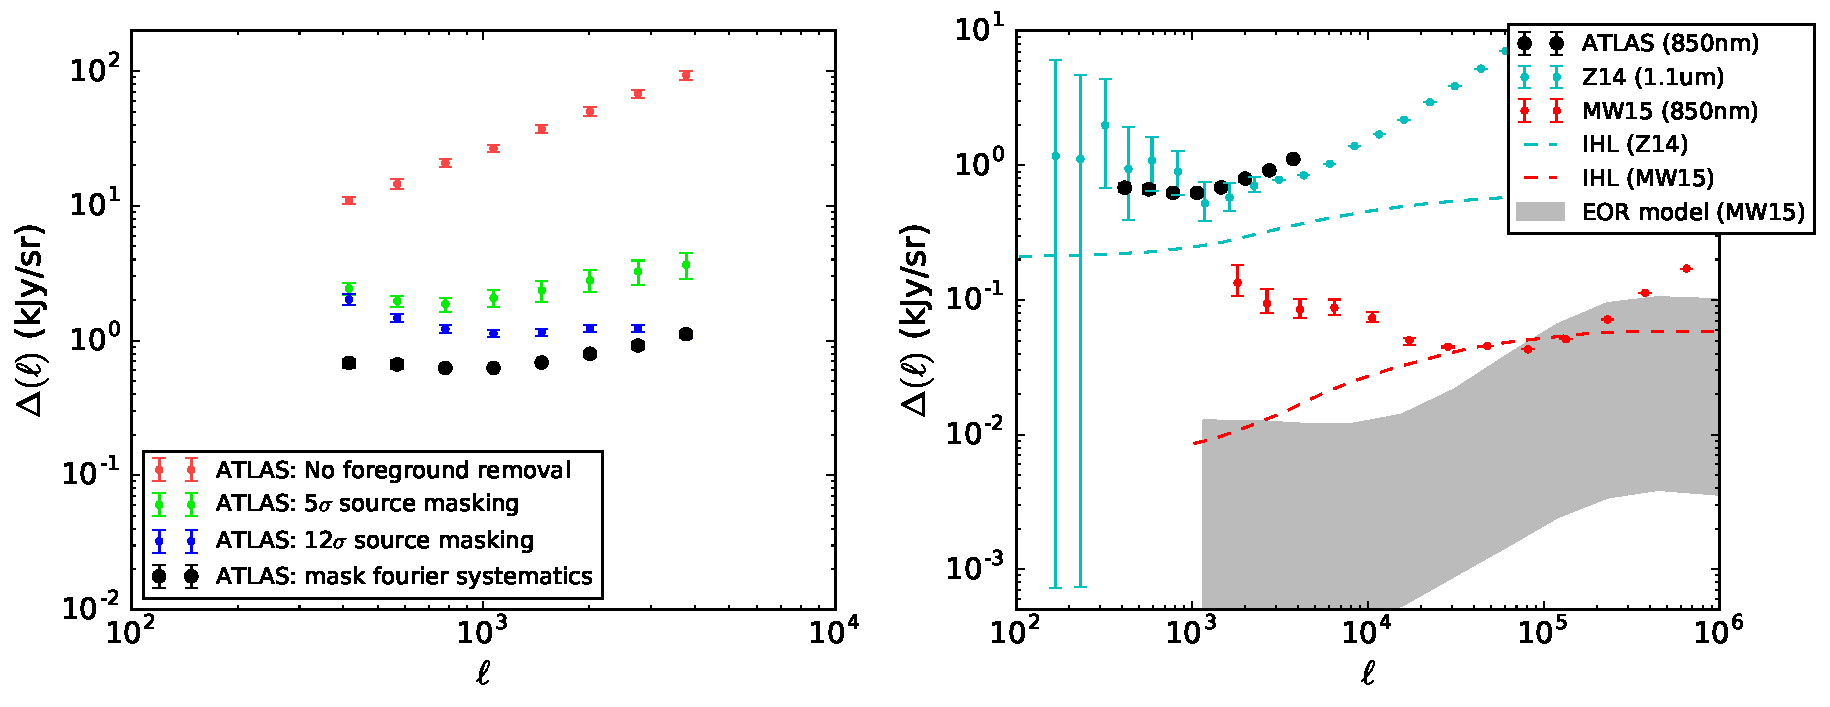
\includegraphics[width=3.5in]{images/big_foreground_masking_study_pspecs_2_magoffset=20_56+0_274.pdf}
\caption{Power spectra of our ($850\pm75$)\,nm broad band ATLAS images after various stages of foreground removal as described in Sec. \ref{sec:resirfg}. The error bars show the sample variance noise estimated by the standard deviation over our four $4^\circ$ fields (see Fig. \ref{fig:surveyoverview}). Black dots show our final infrared anisotropy power spectrum after all stages of foreground removal, and gray crosses show the measurements at ($1100\pm250$)\,nm from \citet{zemcov14}. The black dashed line at the bottom shows the predicted EOR contribution to the infrared anisotropies from \citet{zemcov14}.}
\label{fig:bigfgmaskingstudypspecs}
\end{figure}

Using this estimator, we calculate the power spectrum after each stage of masking and plot the average the average spectrum over all four deep ATLAS fields in Fig. \ref{fig:bigfgmaskingstudypspecs}. We take the standard deviation over the different fields as the error bars, due to sample variance. The power spectrum of all 850\,nm sources, masking only saturated regions, rises as $\ell^1$ (red dots), as expected for poisson source counts when the power spectrum is plotted as $\Delta=\sqrt{\ell^2C_\ell/2\pi}$. Masking sources out to $5\sigma$ removes two orders of magnitude in power (green dots), and masking out to $12\sigma$ and above 70\,kJy/sr over the background removes a factor of a few more in power (blue dots). Lastly, excluding modes with $|\ell_x|<200$ or $|\ell_y|<200$ gives our final 850\,nm anisotropy spectrum (black circles). We note that increasing any of the masking parameters introduced here in this section does not significantly alter these results. Increasing the masking radius around saturated pixels, for instance, results in masking of more coarse pixels, but removes negligible additional power from these residual spectra. 

Our final residual power spectrum agrees well with the CIBER measurements (gray crosses). Below $\ell\sim1000$, both sets of measurements flatten out, though our  four 4$^\circ$ fields give us much more precision than CIBER's $1^\circ$ field of view. At larger ell, both spectra turn upward  and track each other very well with slight gain offset. Our $(850\pm75)$\,nm spectra have $\sim40\%$ more power at these $\ell$ than the CIBER's $(1100\pm250)$\,nm, not necessarily unexpected given than they cover different bands.

\citet{zemcov14} compare the power averaged over $500<\ell<2000$ in their two bands (1.1\,$\mu$m and 1.5\,$\mu$m, each with 0.5\,$\mu$m bandwidth) with longer wavelength measurements up to 4.5\,$\mu$m by \citet{cooray12,kash3,matsumoto11}. They find these measurements fit a Rayleigh-Jeans spectrum. The turnover of this spectrum in the optical or near infrared would give clues as to the source population giving rise to these infrared anisotropies. We integrate the residual fluctuation power in our $850\pm75$\,nm band over the matching range in $\ell$ and find a mean RMS fluctuation power of $\langle\Delta(\ell)\rangle_{500<\ell<2000}=0.70\pm0.02$\,kJy/sr \footnote{These units result from taking the intensity field to be $I_f$.}, equal to $2.48\pm0.07$\,nW/m$^2$/sr \footnote{These units result from taking the intensity field to be $\lambda I_\lambda$, as in \citet{zemcov14}.}. This measurement deviates at the $40\sigma$ level from the 850\,nm Rayleigh-Jeans prediction of 5.5\,nW/m$^2$/sr, indicating that this is the first observation of a significant deviation from the Rayleigh-Jeans spectrum, which is likely starting to turn over towards. \citet{zemcov14} observed weak evidence for this with their measurements at 1.1\,$\mu$m and 1.6\,$\mu$m, but their smaller field of view ($\sim1$ deg sq.) limited their sensitivity to these angular scales, and their measurements deviate from the Rayleigh-Jeans prediction at only the 1$\sigma$ level. 

\subsection{Modeling the 21\,cm--Ly$\alpha$ cross spectrum}
\label{sec:modelingthecrossspectrum}

\begin{figure*}[h]
\centering
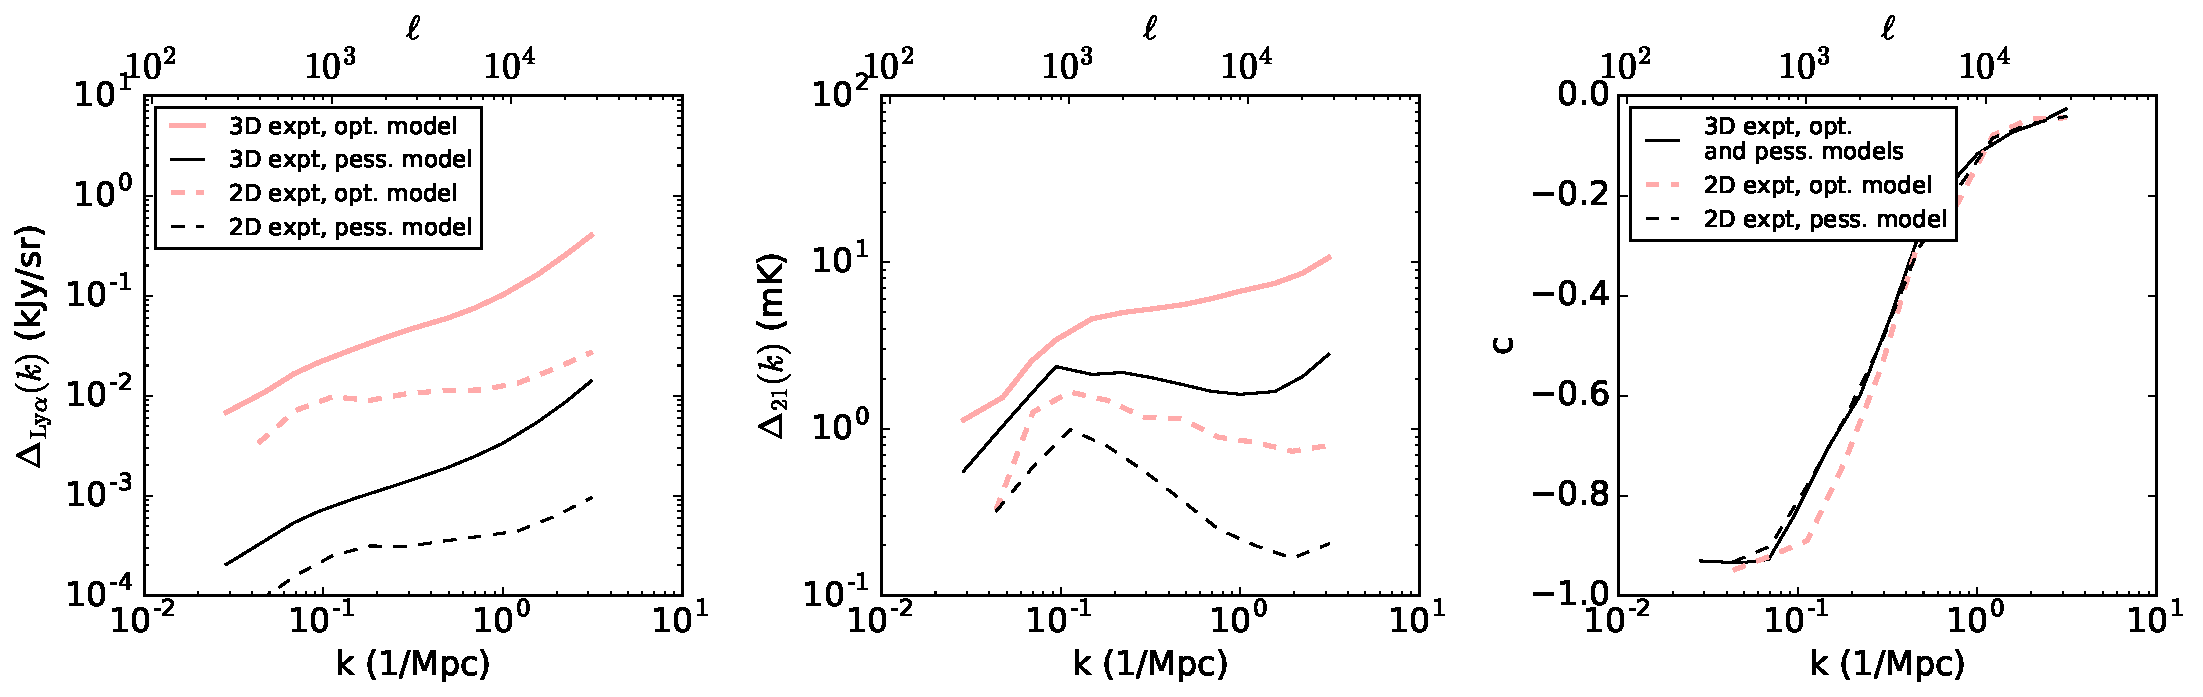
\includegraphics[width=7in]{images/spectra3D_to_2D.pdf}
\caption{As described in Sec. \ref{sec:modelingthecrossspectrum}, we identify optimistic and pessimistic Ly-$\alpha$ (top left) and 21\,cm (top center) 3D power spectra from \citet{Gong2014} and \citet{PoberNextGen}, respectively, and use the coherence function from \citet{Heneka2016} (top right) for both scenarios. We then simulate approximate cubes assuming gaussian statistics, average them over frequency, and plot the angular power spectra of Ly-$\alpha$ (bottom left) and 21\,cm emission (bottom center), and their coherence functions (bottom right). Power on short angular scales ($\ell\gtrsim10^4$) is suppressed by a factor of $\sim100$ (in power units), while power on longer angular scales ($\ell\gtrsim10^4$) is suppressed by only a factor of $\sim2$. This indicates that there remains significant observable signal in broad band 21\,cm--Ly-$\alpha$ cross spectrum observations. }
\label{fig:spectra3Dto2D}
\end{figure*}

Before turning to 21\,cm--Ly-$\alpha$ cross spectrum measurements from our 185\,MHz and 850\,nm images, we generate optimistic and pessimistic theoretical cross spectra for comparison. We simulate 21\,cm and Ly-$\alpha$ cubes using 21\,cm power spectra from \citet{PoberNextGen}, Ly-$\alpha$ power spectra from \cite{Gong2014}, and the coherence between the two fields from \citetext{Heneka2016}. Combining simulations from all these sources allows us to better estimate the modeling uncertainty. Future work is needed to more self-consistently model these fields and their correlation over a range of possible reionization scenarios.  

\citet{Gong2014} model the Ly-$\alpha$ cross spectrum and plot an uncertainty region over a range of likely values of escape fraction of ionizing photons, fraction of radiation emitted at Ly$\alpha$, star-forming rate, and IGM clumping factor (their Fig. 1). We take the upper and lower edges of their uncertainty region as our optimistic and pessimistic power spectra, respectively. 

Similarly, \citet{PoberNextGen} simulate 21\,cm power spectra over a range of reionization scenarios with various values of ionizing efficiency ($\zeta$) (including the escape fraction), the minimum halo virial temperature ($T_\text{ir}$), and the ionizing photon mean free path in the IGM ($R_\text{mfp}$). Whether the signal at our redshift of interest ($z=7$) is large or not depends mostly on whether reionization is already largely finished by that time or not. So we take as our pessimistic model the $z=8$ power spectrum of the ($\zeta =31.5$, $T_\text{vir}=1.5\times10^4$\,K, $R_\text{mfp}=30$\,Mpc) scenario, whose reionization midpoint is $z=9.5$. We take as our optimistic model a late reionization scenario the model with $T_\text{vir}=3\times10^5$\,K (other parameters unchanged), whose reionization midpoint is $z=5.5$. 

From these power spectra and coherence functions, we generate approximate 21\,cm and Ly-$\alpha$ cubes assuming gaussian statistics. The simulated cubes have (1\,Mpc)$^3$ resolution over a (218\,Mpc)$^3$ volume at $z=7$, corresponding to $\Delta z=0.6$ and 0.4' angular resolution. Our 21\,cm and Ly-$\alpha$ cubes have units of mK and kJy/sr, respectively, and we average them in the line of sight direction to produce broad band images.

We plot the original 3D spherically averaged power spectra and coherence function in top panel of Fig. \ref{fig:spectra3Dto2D}, and the computed 2D power spectra from the line-of-sight averaged cubes, as well as their coherence, in the bottom panel. The 3D power spectra are plotted as $\Delta(k)=\sqrt{P(k)k^3/2\pi^2}$, while the 2D spectra are plotted as $\Delta(\ell)=\sqrt{C_\ell \ell(\ell+1)/2\pi}$. As expected, line of sight averaging tends to remove power on short spatial scales (compared to the line of sight depth of the cube), but it acts similarly on both cubes, so the coherence function is preserved. Note that the cross spectrum $\Delta_{12}$ is defined in terms of the coherence as $\Delta_{12}=c\sqrt{\Delta_1\Delta_2}$ for both the 3D and 2D cases, and we use the same coherence function from \citet{Heneka2016} in the optimistic and pessimistic scenarios.


\subsection{Limits on the 21\,cm--Ly$\alpha$ cross spectrum}

Having characterized the residual sky power spectrum at 185\,MHz and 850\,nm after the best foreground masking and subtraction permitted by our datasets, we now search for a correlation between these radio and foreground residuals. To account for the non-uniform $uv$ sampling of the MWA image as well as for the image space masking of the ATLAS image, we again use the optimal quadratic estimator. In Appendix \ref{sec:optimalestimatorforcrossspectrum} we show that with the approximation that the correlation between the two images is small, the proper extension of the optimal quadratic estimator from the auto spectrum case to the cross spectrum case is given by
\begin{equation}
q_\alpha \approx (\xb_{21}-\langle\xb_{21}\rangle)^t \Cb_{21}^{-1} \Cb_{,\alpha}\Cb_\IR^{-1}(\xb_\IR-\langle\xb_\IR\rangle)
\end{equation}
\begin{equation}
\Fb_{\alpha\beta}\approx\text{tr}\left(\Cb_{21}^{-1} \Cb_{,\alpha} \Cb_\IR^{-1}  \Cb_{,\alpha}  \right)	
\end{equation}
where $\Cb_{,\alpha}$ is the same matrix used in Sec. \ref{sec:resirfg}, $\mathbf{x}_{21}$ and $\mathbf{x}_{\IR}$ are the vectors of 21\,cm and IR pixel values. As before we use normalization $\Mb=F^{-1/2}$ in $\pb=\Mb\qb$, and perform a final normalization using the peaks of the window functions $\Wb=\Mb\Fb$. We use the same IR covariance matrix given in Eqn. \ref{eqn:covFTwithmask}, and generate the 21\,cm covariance matrix by writing the diagonal thermal noise covariance matrix fourier space, then fourier transforming it as
\begin{equation}
\label{eqn:C21}
\Cb_{21} = \mathcal{F}^\dagger\text{diag}(|\mathcal{F}\mathbf{w}_{21}|)\mathcal{F}
\end{equation}
where $\mathbf{w}_{21}$ is the vector of pixel values of the image space radio point spread function (i.e., synthesized beam). Though Fig. \ref{fig:respspecspacingsstudy} shows that thermal noise in these broad band images is quite subdominant to the foreground residuals over all $\ell$, it is still beneficial to downweight the most poorly sampled $\vec{\ell}$ modes to mitigate $uv$ gridding artifacts. 

We apply this formalism to each of the four $4^\circ$ deep ATLAS fields shown in Fig. \ref{fig:surveyoverview}, pairing each IR image with the overlapping region of the MWA image cropped from the naturally weighted image. We crop the image space synthesized beam over the same field of view, use it to apply uniform weighting to the cropped MWA image using Eqn. \ref{eqn:uniformweighting}, and use it again to construct $\Cb_{21}$ in Eqn. \ref{eqn:C21}. 

\begin{figure}[h]
\centering
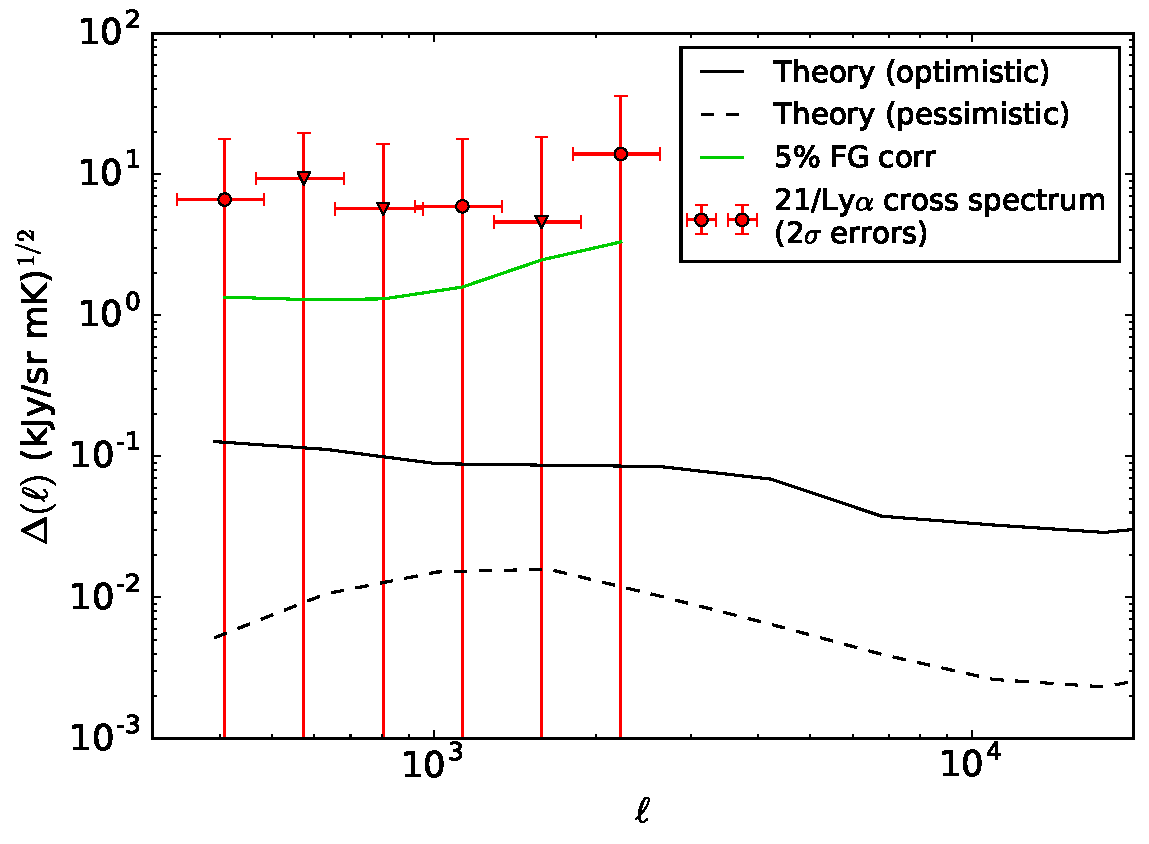
\includegraphics[width=3.6in]{images/mwa_atlas_xspec_with_2Dsimtheory_and_2sigma_errors_6bins.pdf}
\caption{Measured cross spectrum between 185\,MHz and 850\,nm images after our best foreground subtraction and masking (red markers). All are essentially consistent with zero, and roughly half are positive (circles) and negative (triangles), as expected if there is no measurement correlation. Error bars show $2\sigma$ uncertainties, and we take the topes of these error bars as upper limits on the cross spectrum of 21\,cm--Ly$\alpha$ emission from the EOR. We a lowest upper limit of $\Delta_{21,\text{Ly}\alpha}<13.3\,(\text{kJy/sr}\cdot \text{mK})^{1/2}$ (95\%) at $\ell\sim400$. Solid and dashed black lines show the optimistic and pessimistic models derived in Sec. \ref{sec:modelingthecrossspectrum}. Solid, dashed, and dotted blue lines show the predicted sensitivities for improved experiments.}
\label{fig:resxspec}
\end{figure}

In Fig. \ref{fig:resxspec} we plot the resulting cross spectrum (red markers) averaged over all four fields with $2\sigma$ error bars. All are essentially consistent with zero, and roughly half the estimated bandpowers are negative (triangles) and positive (circles), as expected if there is no measured correlation. Our bins are evenly spaced in $\log \ell$, and it is beneficial to overlap them slightly since our normalization matrix $M\sim F^{-1/2}$ ensures bin errors are always uncorrlated. We take the tops of the error bars as 95\% upper limits on the cosmological cross spectrum of 21\,cm and Ly$\alpha$ emission from the EOR, achieving a strongest upper limit of $\Delta_{21,\text{Ly}\alpha}<13.3\,(\text{kJy/sr}\cdot \text{mK})^{1/2}$ (95\%) at $\ell\sim400$. 

The cross spectrum uncertainty due to sample variance noise of residual foregrounds scales approximately as $d\Delta_{21,\IR}\propto f_{21,\text{FG}}^{1/2}d\theta/\theta_{\text{FOV}}$, where $f_{21,\text{FG}}$ is the fraction of remaining 21\,cm foreground power, $d\theta$ is the pixel resolution, and $\theta_{\text{FOV}}$ is the field of view. Our MWA/ATLAS experiment has ($f_{21,\text{FG}}\approx0.1$, $d\theta=6'$, $\theta_{\text{FOV}}=8^\circ$). We plot the predicted sensitivities for improved experiments with (0.1, $0.3'$, 8$^\circ$) (solid blue), (0.01, $0.3'$, 8$^\circ$) (dashed blue), and (0.01, $0.3'$, 40$^\circ$) (dotted blue). \citet{zemcov14,cooray12} argue that the remaining IR foreground is largely due to intrahalo light around already masked sources, and cannot be masked without removing essentially all pixels in the image. We thus do not assume that IR foreground subtraction can be improved.

We find that after increasing the image resolution (of the 21\,cm image) by $20\times$ (to 0.3') and reducing its fractional foreground residuals by $10\times$ (to 0.01), a tenuous detection of the optimistic 21\,cm--Ly$\alpha$ cross spectrum is possible at $\ell<700$. Widening the field of view (of the IR image) by a factor of $5\times$ (to $40^\circ$) permits significant detections at $\ell<1500$. In all these cases, the cross spectrum remains out of reach in the pessimistic scenario, though ruling out the optimistic scenario would significantly constrain reionization models.

\section{Discussion}

NEED TO WRITE THE DISCUSSION SECTION

\begin{acknowledgments}
We acknowledge helpful discussions on optimal quadratic estimators with Adrian Liu, Josh Dillon, and Aaron Ewall-Wice. 
Our analysis code is publicly available at \ULurl{https://github.com/abrahamneben/21cmIRxcor}
\end{acknowledgments}

\appendix

%\section{Power spectrum of photon shot noise}
%\label{sec:Pshot}

%In Sec. \ref{sec:resirfg} we measure the maximum airglow to be $I_\text{air}=5\times10^3$ kJy/sr, and in this appendix we calculate the power spectrum of this photon shot noise. We must observe that the mean number of photons collected by a pixel during each observation is $\langle N_\text{ph}\rangle=I_\text{air}At_\text{int} \Delta f d\theta^2/hf$, where $A=(0.5\,\text{m})^2$ is the collecting area of ATLAS, $t_\text{int}=30\,$sec, $\Delta f$ and $f$ are the frequency bandwidth and center frequency of I band, and $d\theta$ is the pixel size. The passband has $\Delta\lambda=150\,$nm and $\lambda=800\,$nm. 
%
%The shot noise contribution to the power spectrum is given by
%\begin{equation}
%C_{\IR, \shot}(\vec{\ell}) = \left\langle\left|\sum_{m,n}I_\shot(m,n)e^{-2\pi i(ma+nb)/N}\right|^2\right\rangle \frac{d\theta^2}{N^2}
%\end{equation}
%where $I_\shot(m,n)\equiv I(m,n)-\langle I(m,n)\rangle$ denotes the photon shot noise contribution to pixel (m,n), and $N$ is the number of pixels on each side of the square image. Then using the fact that the shot noise is uncorrelated between different pixels, we find
%\begin{equation}
%C_{\IR, \shot}(\vec{\ell}) = \sum_{m,n}\langle I^2_\shot(m,n)\rangle \frac{d\theta^2}{N^2}
%\end{equation}
%Note that $I(m,n)=N_\text{ph}(m,n)hf/\Delta f A t_\text{int}d\theta^2$ and $\langle N_\text{ph}^2\rangle = \langle N_\text{ph}\rangle$, so we have
%\begin{equation}
%C_{\IR, \shot}(\vec{\ell}) = \langle N_\text{ph}\rangle \left(\frac{hf}{\Delta f A t_\text{int}d\theta^2}\right)^2 d\theta^2
%\end{equation}
%
%\begin{equation}
%C_{\IR, \shot}(\vec{\ell}) =\frac{I_\text{air}h\lambda}{\Delta \lambda A t_\text{int}}
%\end{equation}

\section{Relation between the power spectrum of image cubes and broadband images}
\label{sec:pspecrelation}

We focus in this paper on the spherical power spectrum of broadband images, $C_\ell$,  instead of that of image cubes, $P(\vec{k})$, as 21\,cm observations have focused on. Here we work out the approximate relation between the two over small fields of view (i.e., for large $\ell$) to facilitate comparison with past 21\,cm power spectrum results. In particular, we calculate the scaling factor $B$ relating the purely transverse modes of the power spectrum $P(k_\perp,k_\parallel=0)$ of a image cube $I(\theta_x,\theta_y,f)$ to the spherical power spectrum of a broad band image $C_\ell$ as
\begin{equation}
P(k_\perp,k_\parallel=0) = B C_{\ell(k_\perp)}
\end{equation}

Using the fourier transform convention discussed in Sec. \ref{sec:pspecconventions}, the left side of the equation is given by
\begin{equation}
P(k_\perp,k_\parallel=0) = \frac{1}{N_\perp^2 N_\parallel dV}\langle|\tilde{I}(k_x,k_y,k_\parallel=0)|^2\rangle
\end{equation}
where $N_\perp\equiv N_x=N_y$ is the number of pixels in each of the two transverse dimensions of the image cube, and $N_\parallel$ is the number of pixels in the line of sight (ie, frequency) dimension. The comoving pixel volume is $dV = (D_c d\theta)^2 (\Delta D_c/N_\parallel)$, where $D_c$ is the line of sight comoving distance from the present day to the center of the cube, and $\Delta D_c$ is the comoving line of sight thickness of the cube. Lastly, recall that $k_\perp$ is related to $k_x$ and $k_y$ as $k_\perp=\sqrt{k_x^2+k_y^2}$.

Now substituting the definition of the fourier transform, we find

\begin{equation}
P(k_\perp,k_\parallel=0) =\frac{1}{N_\perp^2 N_\parallel dV}\left\langle\left|dV\sum_{\theta_x,\theta_y,f}I(\theta_x,\theta_y,f)e^{iD_c(k_x\theta_x+k_y\theta_y)}\right|^2\right\rangle
\end{equation}

Simplifying and writing this in terms of the broadband image $I_{\Delta f}(\theta_x,\theta_y)\equiv\frac{1}{N_\parallel}\sum_f  I(\theta_x,\theta_y,f)$, we find

\begin{equation}
P(k_\perp,k_\parallel=0) =(D_c^2 \Delta D_c)
\frac{d\theta^2}{N_\perp^2}\left\langle\left|\sum_{\theta_x,\theta_y}I_{\Delta f}(\theta_x,\theta_y)e^{iD_c(k_x\theta_x+k_y\theta_y)}\right|^2\right\rangle
\end{equation}

Now denote $k_x=a\cdot dk$, $k_y=b\cdot dk$, $\theta_x=m\cdot d\theta$, and $\theta_y=n\cdot d\theta$, where $dk = 1/N_\perp D_c d\theta$. 

\begin{equation}
P(k_\perp(\ell(a,b)),k_\parallel=0) =(D_c^2 \Delta D_c)
\frac{d\theta^2}{N_\perp^2}\left\langle\left|\sum_{m,n}I_{\Delta f}(m,n)e^{2\pi i(am + bn)/N_\perp}\right|^2\right\rangle
\end{equation}

Comparing with Equations \ref{eqn:Cldef}, \ref{eqn:elldef}, and \ref{eqn:elldef2}, we see that $B\equiv P(k_\perp,k_\parallel=0)/ C_{\ell(k_\perp)}=D_c^2 \Delta D_c$ and $\ell=D_c k_\perp$.


\section{Extending the optimal quadratic power spectrum estimator to the cross spectrum case}
\label{sec:optimalestimatorforcrossspectrum}

The optimal quadratic estimator formalism presented in Sec. \ref{sec:resirfg} was constructed to estimate the power spectrum of an image with arbitrary pixel sampling and noise properties. In this section we extend this formalism to achieve the same advantages in cross spectrum measurements. 

Consider measurements at two bands over the same set of pixels on the sky, $\xb_1$ and $\xb_2$, each column vectors with $N$ elements. Let us combine these together into a single column vector containing all measurements as $\xb=\left(\begin{matrix}\xb_1 \\ \xb_2  \end{matrix}\right)$, whose covariance is given by 

\begin{equation}
\Cb\equiv  \langle\xb\xb^\dagger\rangle-\langle\xb\rangle\langle\xb^\dagger\rangle=\left(\begin{matrix}\Cb_1 & \Cb_{12} \\ \Cb_{12}^\dagger & \Cb_2   \end{matrix}\right)
\end{equation}
and 
\begin{equation}
\frac{d\Cb}{dp_{12}^\alpha}=\left(\begin{matrix}\mathbf{0} & \Cb_{,\alpha}\\ \Cb_{,\alpha}^\dagger & \mathbf{0}   \end{matrix}\right)
\end{equation}
$\Cb_1$ and $\Cb_2$ depend only on the auto power spectra of the different fields; only $\Cb_{12}$ depends on the cross spectrum. Said another way, $C_{,\alpha}$ is the same matrix used in Sec. \ref{sec:resirfg}, but used here in the off-diagonal parts of $d\Cb/dp_{12}^\alpha$ so as to capture the cross products between the two fields\footnote{One might object to our form of $d\Cb/dp_{12}^\alpha$, arguing that artificially limiting ourselves to cross products between the two fields is tantamount to throwing a significant amount of the information contained in the data sets, and thus our estimator cannot be optimal. There are certainly situations in which this would be the case. If we had some theory of how each field was related to the matter density field of the universe, then both the auto-products and cross-products contain similar information. However we take an empirical approach where we assume we know nothing about either field but want to know their correlation. Only the cross products contain that information.}. And as before, the unnormalized estimator $q_\alpha$ of the power in band $\alpha$ is given by
\begin{equation}
q_\alpha = \frac{1}{2}(\xb-\langle\xb\rangle)^\dagger \Cb^{-1} \frac{d\Cb}{dp_{12}^\alpha}\Cb^{-1}(\xb-\langle\xb\rangle)
\end{equation}
and the elements of the Fisher matrix are
\begin{equation}
\Fb_{\alpha\beta}=\frac{1}{2}\text{tr}\left(\Cb^{-1} \frac{d\Cb}{dp_{12}^\alpha} \Cb^{-1}  \frac{d\Cb}{dp_{12}^\beta}  \right)	
\end{equation}

In the case where the correlation between the two fields is expected to be weak, and we are primarily interested in setting an upper limit, we can get a significant speedup by approximating $\Cb_{12}\approx0$ in our guess covariance. The expressions for $q_\alpha$ and $F_{\alpha\beta}$ then simplify to:
\begin{equation}
q_\alpha \approx (\xb_1-\langle\xb_1\rangle)^\dagger \Cb_1^{-1} \Cb_{,\alpha}\Cb_2^{-1}(\xb_2-\langle\xb_2\rangle)
\end{equation}
\begin{equation}
\Fb_{\alpha\beta}\approx\text{tr}\left(\Cb_1^{-1} \Cb_{,\alpha} \Cb_2^{-1}  \Cb_{,\alpha}  \right)	
\end{equation}


%% The reference list follows the main body and any appendices.
%% Use LaTeX's thebibliography environment to mark up your reference list.
%% Note \begin{thebibliography} is followed by an empty set of
%% curly braces.  If you forget this, LaTeX will generate the error
%% "Perhaps a missing \item?".
%%
%% thebibliography produces citations in the text using \bibitem-\cite
%% cross-referencing. Each reference is preceded by a
%% \bibitem command that defines in curly braces the KEY that corresponds
%% to the KEY in the \cite commands (see the first section above).
%% Make sure that you provide a unique KEY for every \bibitem or else the
%% paper will not LaTeX. The square brackets should contain
%% the citation text that LaTeX will insert in
%% place of the \cite commands.

%% We have used macros to produce journal name abbreviations.
%% AASTeX provides a number of these for the more frequently-cited journals.
%% See the Author Guide for a list of them.

%% Note that the style of the \bibitem labels (in []) is slightly
%% different from previous examples.  The natbib system solves a host
%% of citation expression problems, but it is necessary to clearly
%% delimit the year from the author name used in the citation.
%% See the natbib documentation for more details and options.

%\bibliography{xcor_paper}
\bibliography{xcor_paper_new}


\end{document}
